%% main.tex --- Bucket Brigade workshop paper (v8 draft)
%%
%% v8 integrates the three post-v7 results (repo issue #462; PRs #455,
%% #456, #460; issues #443, #444, #445):
%%   - \S5 (social-trap hardness): the budget-scaling ladder (issue #444,
%%     PR #460). het_ppo at 16x budget is the first `escaped_trap` verdict
%%     on rest_trap-v1 (trailing-5 mean 307.83, seed-bootstrap 95% CI
%%     [305.00, 310.71], lower bound clearing the 304.31 random-anchor
%%     upper bound by +0.69/step; robust across 300/300 bootstrap
%%     configurations and to a t-interval [304.67, 310.99]). The flip is
%%     variance-driven -- no dose-response on the mean (306.26 / 307.66 /
%%     307.83) -- so the hardness headline is sharpened, not weakened:
%%     budget buys precision, not performance. The anchor table gains the
%%     16x row; the marginality/CRN-multiplicity caveats of
%%     docs/PAPER_RESULTS.md section 9 are carried.
%%   - \S5 (equilibrium characterization): rest_trap symmetric-DO cycling
%%     confirmed and characterized (issue #445, PR #455): the
%%     battery-seeded retry ran 50/50 iterations without converging (min
%%     improvement 11.79 vs eps 0.01), the final mixture is exploitable by
%%     >= 407.50/episode, the genome-mapped specialist team is exploitable
%%     at every position (+605 to +870/episode). The asymmetric FRx3+FF NE
%%     (2984.04/episode) stands; equilibrium coverage is now 12/12 frozen
%%     scenarios (11 converged + 1 exploitability-bounded cycling entry).
%%   - \S4 (trainability/noise): 20-seed noise buy-down (issue #443,
%%     PR #456). CI half-widths on gap_closed_ne shrink 2.00-3.64x
%%     (median 2.65) on the 8 partially-k*-stratified cells; 0/8 verdicts
%%     flip; entropy retirement re-verified at n=20 (rho = 0.109,
%%     p = 0.56); the k* class test under the partial thrust#259/#268
%%     stratification is not significant (exact MW p = 0.43) and remains
%%     blocked on thrust#269.
%%   - Open threads cited in \S3/\S6: repo issue #459 (are the
%%     phase-diagram asymmetric profiles eps-NE under CRN re-evaluation?)
%%     and #461 (superseded v1 recalibration artifact drift).
%% The stale-claim audit table for this revision is committed alongside at
%% stale_claims_audit.md.
%%
%% v7 integrated the July-2026 session results (repo issue #446): the
%% retired entropy predictor + beta-invariance impossibility argument in
%% \S4, the new \S5 social-trap section, the #442 beta-inertness
%% corrections, and the expanded reproducibility subsection. v6 landed the
%% v5-reviewer/auditor punch list. v5 inlined the memo placeholders as
%% Appendices A/B. v8 preserves all of those changes.
%%
%% Authored via anvil:pub. Compiles with pdflatex + bibtex against the
%% anvil-paper class shipped at .anvil/skills/pub/templates/anvil-paper.cls.
%% Figure 2 is rendered offline by figures/src/recalibrated_heatmap.py and
%% reads from
%% experiments/p3_specialization/phase_diagram_ppo_v2/recalibrated_verdict.json.

\documentclass{anvil-paper}

% Extra packages used by this paper specifically.
\usepackage{tikz}
\usetikzlibrary{patterns}
\usepackage{array}

\title{Bucket Brigade: A Parametric Cooperative-Competitive Benchmark with
Computable Nash Equilibrium Structure}
\author{Robb Walters \\ 2AM Logic}
\date{\today}

\begin{document}
\maketitle

\begin{abstract}
Canonical cooperative-MARL benchmarks (Overcooked, Hanabi, SMAC, Melting Pot,
MAgent, PettingZoo) trade equilibrium transparency for environment richness:
their state spaces are large enough that no Nash equilibrium is computable, so
when a new algorithm beats PPO on Overcooked the reader cannot tell whether
the algorithm has converged to the ``right'' joint policy or merely to a
Pareto-different one. \emph{Bucket Brigade} inverts this trade. It is a finite
parametric cooperative-competitive stochastic game on a ring of houses whose
per-agent action space at the minimal parameterization is~$8$, whose state
space is~$2304$ states, and whose three load-bearing scalars~$(\beta,\kappa,c)$
control equilibrium structure continuously across cells. We give the
environment specification, derive closed-form boundary inequalities for the
three Nash-equilibrium regimes (symmetric all-Work, asymmetric 1-Worker,
no-pure-NE collapse) via a single-house mean-field reduction, and report
empirical agreement between predicted and PPO-realised verdicts on a
$39$-cell phase diagram ($\beta{\times}\kappa{\times}c$). The reduction
correctly predicts the qualitative phase order
(collapse~$\to$~symmetric~$\to$~mixed~$\to$~asymmetric); its
$\beta$-independence prediction turns out to hold \emph{by construction}
in the sweep's bernoulli extinguish mode (fire spread never fires under
the canonical phase order), so cross-$\beta$ residuals measure solver
noise rather than testing the reduction. The $39$-cell grid surfaces a
fourth empirical
class~--~\textsf{mixed} ($9/37$ PPO cells, both pure NE coexist)~--~which
the closed-form bound does not predict at the higher-$c$ regime where it
emerges. The trainability sweep ($37$ cells, $50$~iter${\times}2048$~steps,
$4$~seeds) recovers the same ordering under a per-cell NE-anchored metric:
$\texttt{gap\_closed\_ne}$ is largest on \textsf{symmetric\_only}~$(0.180)$,
smaller on \textsf{mixed}~$(0.107)$ and \textsf{asymmetric\_only}~$(0.059)$,
and negative on \textsf{no\_convergence}~$(-0.049)$. A
$4{\times}$-budget sweep on the no-convergence cells worsens
$\texttt{gap\_closed\_homogeneous}$ to~$-0.108$, indicating PPO's failure on
those cells is structural rather than budget-limited. We also report a
negative result: conditional entropy of the cell's NE profile does not
predict per-cell gap closure (Spearman $\rho{=}0.007$), and since the
converged NE profile is identical across $\beta$ within each
$(\kappa,c)$ column while trainability varies, \emph{no} statistic of
the NE profile can explain the within-column variance; a $20$-seed
noise buy-down shrinks CI half-widths $2.0$--$3.6{\times}$ on an
$8$-cell subset while flipping none of the $8$ trainability verdicts
and re-verifying the entropy retirement, and the replacement
coordination-threshold ($k^{*}$) hypothesis remains unvalidated (its
class test is insignificant under a partial stratification). On the
social-trap scenario \texttt{rest\_trap-v1}, whose frozen equilibrium
is team-suboptimal by construction~--~and whose equilibrium
characterization is now closed: two independent symmetric double-oracle
runs cycle, the seeded run's final mixture is exploitable by
${\geq}407.5$/episode, and the asymmetric equilibrium stands~--~an
all-scripted specialist team scores $386.6$/step where $20$-seed PPO
at the standard budget reaches $306.3$~--~statistically
indistinguishable from uniform-random play
($302.9$)~--~a machine-verdicted ${\approx}80$/step learnability gap
that gives the benchmark a measured, currently-uncaptured headroom
target. A $4{\times}$/$16{\times}$ budget-scaling ladder sharpens the
hardness statement: exactly one configuration ($16{\times}$
heterogeneous PPO) crosses the pre-registered escape threshold
marginally (CI lower bound $305.00$ vs.\ the $304.31$ random-anchor
upper bound), with no dose-response on the mean~--~budget buys
seed-level precision, not performance, and the mean uplift stays at
${\approx}6\%$ of the scripted headroom. The quantitative
$\kappa$-thresholds of the reduction disagree with the equilibrium solver
by $3$--$10\times$; we own this gap and attribute it to ring-locality,
per-agent ownership rewards, and the heuristic-strategy approximation. We position Bucket Brigade as a \emph{methodological
complement} to the surveyed benchmarks, not a replacement: it is the only
published parametric MARL game where the question ``did the algorithm
converge to the right equilibrium?'' admits a ground-truth answer.
\end{abstract}

\section{Introduction}
\label{sec:intro}

Multi-agent reinforcement learning evaluates new algorithms against benchmarks
whose Nash-equilibrium structure is not characterizable in closed form.
Overcooked-AI~\citep{overcooked2019}, DeepMind's Melting
Pot~\citep{meltingpot2021}, the Hanabi
Challenge~\citep{hanabi2020}, SMAC and SMACv2~\citep{smac2019,smacv2_2023},
MAgent~\citep{magent2018}, and the PettingZoo MPE
suite~\citep{pettingzoo2021} between them cover small cooperative
coordination, partial observability, scripted-opponent micromanagement, and
population-scale competition. None of them ship with a method that produces
the equilibrium strategy profile of the as-designed environment. When PPO
fails to learn a coordinated policy on Overcooked, the community is left to
debate whether the failure is the algorithm or the absence of a clean
attractor for self-play; neither hypothesis can be rejected because no oracle
exists for ``what should the learned policy look like.''

We introduce \emph{Bucket Brigade}, a finite parametric cooperative-competitive
stochastic game designed to invert this trade. At its minimal parameterization
the state space is $2304$~states and the per-agent action space is~$8$, so the
one-shot stage game is enumerable and standard equilibrium-computation tools
actually run. Across a smooth three-scalar parameter family~$(\beta,\kappa,c)$
the equilibrium structure transitions from symmetric all-Work to asymmetric
1-Worker (the textbook free-rider problem) to no-pure-NE collapse, with a
fourth empirically-observed regime~--~\textsf{mixed}, where both symmetric
and asymmetric pure NE coexist~--~appearing at high~$\kappa$ on the
higher-$c$ rows of the grid. The ground-truth target for each parameter cell
is known, so a failed PPO run is attributable to the algorithm rather than
to ambiguity about what convergence would mean. The pitch is exactly a
\emph{methodological complement} to the six canonical benchmarks above: those
exist for studying open-ended cooperation, generalization, and scale; Bucket
Brigade exists for studying equilibrium-convergence quality on a controlled
grid.

\paragraph{Contributions.} (1)~A self-contained formal specification of the
Bucket Brigade game~(\S\ref{sec:env}), recovering Volunteer's Dilemma, the
$N$-player Public Goods game, and Stag Hunt as named limits.
(2)~Closed-form boundary inequalities~(\S\ref{sec:ne}) for the three NE
regimes via a single-house mean-field reduction, together with an explicit
accounting of where the closed-form thresholds disagree with empirics and
where a fourth (\textsf{mixed}) class emerges that the bound does not
predict. (3a)~A protocol and the first empirical
results~(\S\ref{sec:trainability}) testing PPO trainability against the
NE phase diagram on the full~$37$-cell grid: the PPO ordering recovered
by a per-cell NE-anchored metric is consistent with the analytical
prediction
\textsf{symmetric}~$>$~\textsf{mixed}~$>$~\textsf{asymmetric}~$>$~%
\textsf{collapse}, and a separate~$4{\times}$-budget sweep on the
no-convergence cells worsens, not improves, gap-closure~--~PPO's
failure on those cells is structural, not budget-limited.
(3b)~The per-cell NE-anchored metric itself, surfaced as a standalone
methodological contribution: on this paper's data, the previously-used
single-cell baseline inverts the per-class ordering (\S\ref{sec:trainability}),
so per-cell calibration is not a cosmetic refinement but a necessary
correction for cross-cell PPO comparison whenever the random-policy
return varies across cells.
(3c)~A negative result on per-cell trainability
predictors~(\S\ref{sec:trainability}): conditional entropy of the
converged NE profile is uncorrelated with per-cell gap closure, and a
$\beta$-invariance argument rules out \emph{every} statistic of the NE
profile as an explanation of within-$(\kappa,c)$-column variance; a
$20$-seed noise buy-down on an $8$-cell subset shrinks CI half-widths
$2.0$--$3.6{\times}$, flips none of the $8$ trainability verdicts, and
re-verifies the retirement, while the replacement
coordination-threshold ($k^{*}$) hypothesis remains unvalidated (class
test insignificant under a partial stratification; the full test is
blocked on a pending per-cell $k^{*}$ artifact).
(4)~A measured social-trap hardness result~(\S\ref{sec:resttrap}): on
\texttt{rest\_trap-v1} a fully-scripted specialist team scores
$386.60$/step against a $302.87$/step uniform-random baseline, while
$20$-seed PPO at the standard budget is statistically indistinguishable
from random and a $16{\times}$-budget run separates from random only
marginally and without mean improvement~--~a machine-verdicted
${\approx}80$/step learnability gap, grounded in a measured anchor
ladder and a pre-registered verdict rule rather than an ad-hoc fraction
gate. The scenario's equilibrium characterization is closed: the
symmetric double oracle cycles across two independent runs (and the
seeded run's final mixture is measurably far from equilibrium), so the
asymmetric equilibrium stands. (5)~An honest
positioning~(\S\ref{sec:related},~\S\ref{sec:discussion}) against the
canonical benchmarks: Bucket Brigade is small and artificial by design,
and is not a substitute for any of them.
Throughout, we treat the analytical NE characterization as ground truth and
the PPO trainability sweep as a falsification test, in that order.

\section{The Bucket Brigade environment}
\label{sec:env}

\paragraph{Players and topology.}
A finite set of agents $\mathcal{I}{=}\{1,\ldots,N\}$ inhabits a cycle graph
$\mathcal{H}{=}\mathbb{Z}/H\mathbb{Z}$ of $H$ houses with neighbour edges. Each
house has status $h_h\in\{\textsc{Safe},\textsc{Burning},\textsc{Ruined}\}$;
\textsc{Ruined} is absorbing. The default ``10-house'' scenario fixes
$H{=}10,N{=}4,T_{\min}{=}12$; the minimal scenario fixes $H{=}2,N{=}4$.

\paragraph{Action and observation.}
Each agent $i$ chooses
$a_{t,i}{=}(a^{\text{house}},a^{\text{mode}},a^{\text{sig}})\in
\mathcal{H}\times\{0,1\}\times\{0,1\}$: a target house, a
\textsc{Work}/\textsc{Rest} bit, and a one-bit broadcast signal observable to
all agents on the next night. Per-agent action cardinality is $4H$ ($8$ at
$H{=}2$; $40$ at $H{=}10$). Joint-action cardinality at the minimal
parameterization is $8^4{=}4096$. Observation is symmetric perfect monitoring
with one-step signal delay: every agent observes the full state plus the
previous joint $(\ell_{t-1},\alpha_{t-1},\zeta_{t-1})$. There is no partial
observability of houses or agent positions; the signal channel is
non-binding cheap talk.

\paragraph{Transition dynamics.}
A single night consists of seven sequential phases applied in a fixed,
load-bearing order: (1)~signal write, (2)~location/mode write,
(3)~extinguish, (4)~burn-out, (5)~spread, (6)~spontaneous ignition,
(7)~reward and termination check. In the extinguish phase, if $w_h(a)$
agents \textsc{Work} at a \textsc{Burning} house, the house transitions to
\textsc{Safe} with probability $1-(1-\kappa)^{w_h(a)}$ (independent-workers
model). Every \textsc{Burning} house that survives the extinguish phase
transitions deterministically to \textsc{Ruined} in the burn-out phase. The
spread phase then ignites \textsc{Safe} neighbours of \textsc{Burning}
houses with probability $\beta$ per edge; under the canonical order, the
burn-out phase has already cleared all \textsc{Burning} sources, so spread is
inert in the within-night dynamics and contagion enters only via the
spontaneous-ignition phase~6 at rate $\rho$. (A contagion-active variant
that swaps phases 4 and 5 is available; the phase-diagram analysis below
uses the canonical order.)

\paragraph{Reward structure.}
The per-agent reward decomposes into three independently-parameterised terms:
a private work/rest cost ($-c$ for \textsc{Work}, $+c_{\text{rest}}{=}0.5$
for \textsc{Rest}; the free-rider gradient is the $c{+}c_{\text{rest}}$
asymmetry), a per-house ownership term ($r_{\text{own}}$ paid on save,
$p_{\text{own}}$ recurring on every \textsc{Ruined} night), and a team
welfare term proportional to the fraction of \textsc{Safe} and
\textsc{Ruined} houses. Ownership is assigned round-robin
($\text{owner}(h){=}h\bmod N$). The asymmetric reward variants in the
calibrated family let $r_{\text{own}},r_{\text{other}},p_{\text{own}},
p_{\text{other}}$ be set per-agent, breaking exchangeability.

\paragraph{Relationship to canonical templates.}
Bucket Brigade recovers, as named limits or restrictions, several textbook
templates: the $N$-player Volunteer's Dilemma at $H{=}1$; the $N$-player
Public Goods game when ownership weights collapse to uniform; Stag Hunt in
the $\kappa{\to}1$ limit; and a free-rider problem at the parameter cells
where the only NE is asymmetric (the ``rest-trap''). Formal proofs and a
complete notation table appear in Appendix~\ref{app:envspec};
\S\ref{sec:env} above is the minimal contract a reader needs to follow
\S\ref{sec:ne}.

\section{Equilibrium structure: closed-form boundaries}
\label{sec:ne}

The central contribution of this paper is a closed-form characterisation of
which Nash-equilibrium structure appears as a function of $(\beta,\kappa,c)$
in the 4-agent game. We derive it via a single-house mean-field reduction
that collapses the $H{=}10$ ring to a representative single house with all
$N{=}4$ agents present, absorbs multi-step contagion and ignition dynamics
into a per-night survival coefficient, and reads off the NE candidates as
algebraic inequalities.

\paragraph{Reduction.}
Fix the \texttt{minimal\_specialization} reward tuple
$W{=}(R_{\text{team}},P_{\text{team}},r_{\text{own}},r_{\text{other}},
p_{\text{own}},p_{\text{other}}){=}(10,10,50,0,100,0)$ and $\rho{=}0.02,
T_{\min}{=}12$. With $k$ workers at the house on a given night, the per-night
ruin probability for an initially-\textsc{Safe} house is
$q(k){=}\rho(1-\kappa)^k$ (under the canonical phase order, where $\beta$
does not enter the leading-order single-night payoff). Integrating the lost
per-house reward stream over $T_{\min}{=}12$ nights and collecting terms
yields
\[
  \mathbb{E}[\text{per-house reward loss}\mid k] = A\cdot\rho\cdot(1-\kappa)^k,
\]
with $A{=}r_{\text{own}}T_{\min}+p_{\text{own}}T_{\min}+P_{\text{team}}
T_{\min}/H{=}1812$ and survival coefficient
$\tilde A{:=}A\rho{=}36.24$. The marginal benefit of adding the $k$-th
worker is $\Delta(k){=}\tilde A\cdot\kappa\cdot(1-\kappa)^k$.

\paragraph{The three NE candidates.}
Writing $c_{\text{gap}}{:=}c+c_{\text{rest}}$ (so $c_{\text{gap}}{=}1.0$ when
the driver sets $c{=}0.5$), the deviation comparisons against the per-night
stage game under stationary opponent policies yield three inequalities.

The \emph{symmetric all-Work} NE exists iff a unilateral deviation from
$k{=}4$ to $k_{-i}{=}3$ does not pay:
\begin{equation}
  \tilde A\cdot\kappa\cdot(1-\kappa)^{3}\;\geq\;c_{\text{gap}}.
  \tag{S}\label{eq:S}
\end{equation}

The \emph{asymmetric 1-Worker} NE exists iff the lone worker prefers
\textsc{Work} ($k_{-i}{=}0$ deviation) and each free-rider prefers
\textsc{Rest} ($k_{-i}{=}1$ deviation):
\begin{equation}
  \tilde A\cdot\kappa\;\geq\;c_{\text{gap}}
  \quad\text{AND}\quad
  \tilde A\cdot\kappa\cdot(1-\kappa)\;<\;c_{\text{gap}}.
  \tag{A}\label{eq:A}
\end{equation}

The \emph{no-pure-NE collapse} regime holds whenever even a lone worker
cannot recover their cost, so neither~\eqref{eq:S} nor~\eqref{eq:A} can be
satisfied:
\begin{equation}
  \tilde A\cdot\kappa\;<\;c_{\text{gap}}.
  \tag{C}\label{eq:C}
\end{equation}

\paragraph{Predicted thresholds.}
Substituting $\tilde A{=}36.24,c_{\text{gap}}{=}1.0$ into~\eqref{eq:S}--%
\eqref{eq:C}: the collapse boundary~\eqref{eq:C} sits at
$\kappa\approx 0.028$; the symmetric NE exists on
$\kappa\in[0.030,0.65]$ via~\eqref{eq:S}; the asymmetric NE exists for
$\kappa\gtrsim 0.972$ via~\eqref{eq:A}. The qualitative phase order
$\kappa$-small$\to$$\kappa$-large is
\textsf{collapse}~$\to$~\textsf{symmetric\_only}~$\to$~\textsf{mixed}~$\to$~%
\textsf{asymmetric\_only}, and the derivation is structurally
$\beta$-independent under the canonical phase order.

\paragraph{Predicted vs.\ observed thresholds.}
The empirical phase diagram, computed by a heterogeneous Double-Oracle
solver over continuous heuristic-parameter strategies on a $39$-cell grid
($\beta\in\{0.1,0.5,0.9\}\times\kappa\in\{0.1,0.3,0.5,0.7,0.9\}\times
c\in\{0.5,1.0,2.0\}$, less six cells in the high-$\kappa\times c{=}0.5$
corner subsumed by the $c{=}1.0$ row; Figure~\ref{fig:phase}), recovers the
qualitative phase order and approximate $\beta$-independence at verdict
level: 12 of the 13 $(\kappa,c)$ rows with $\geq 2$ $\beta$ samples
show an identical verdict across all sampled $\beta$. The single
splitting row is $(\kappa{=}0.9, c{=}0.5)$, where $\beta{=}0.1$
yields \textsf{mixed} while $\beta\in\{0.5, 0.9\}$ yield
\textsf{asymmetric\_only}.

An important caveat, established after the sweep by mechanistic
inspection of the engine (repo issue~\#442): in the bernoulli extinguish
mode the sweep uses, $\beta$-invariance is not merely a leading-order
prediction of the reduction~--~it is \emph{exact by construction}. Under
the canonical phase order the burn-out phase clears every
\textsc{Burning} house before the spread phase runs, so spread is a
guaranteed no-op and, because it draws zero RNG in this mode, the
dynamics \emph{and the RNG stream} are bit-identical across $\beta$.
Verdict-level $\beta$-invariance therefore cannot confirm the reduction;
it is a consistency check on the solver. The useful reading is the
converse: any residual cross-$\beta$ difference at fixed $(\kappa,c)$ is
a direct measurement of double-oracle solver nondeterminism. The lone
splitting row above is exactly such a measurement~--~not an environment
anomaly~--~and the same probe shows the solver's \emph{payoffs} carry
noise as well: at $(\kappa{=}0.9,c{=}0.5)$ the $\beta{=}0.1$ run
returns equilibrium payoff $80.9$ against $72.0$ at
$\beta\in\{0.5,0.9\}$ for the bit-identical environment
(\texttt{experiments/nash/phase\_diagram/results.json}). Equilibrium
\emph{payoff} values from the solver should accordingly be read with an
unquantified solver-noise error bar; verdict classes, which agree on
$12/13$ rows, are more robust. (Whether the solver's converged
asymmetric profiles are themselves $\varepsilon$-NE under
common-random-number re-evaluation is an open question, tracked as repo
issue~\#459.) The grid surfaces \emph{four}
empirical classes: in addition to \textsf{symmetric\_only}~($n{=}12$),
\textsf{asymmetric\_only}~($n{=}11$), and \textsf{no\_convergence}~($n{=}6$),
a \textsf{mixed} class~($n{=}10$) appears in which the solver returns both
symmetric all-Work and asymmetric 1-Worker profiles as un-deviable,
primarily at $\kappa{=}0.9$ on the $c{\geq}1$ rows and at $\kappa{=}0.5,
c{=}2.0$. The closed-form bound~\eqref{eq:S}--\eqref{eq:C} does not predict
this fourth class at the higher-$c$ regime where it emerges: the derivation
pivots on $\tilde A\kappa(1-\kappa)^{k}$ being above or below
$c_{\text{gap}}$, which excludes the simultaneous-existence pattern.
Tightening the reduction to predict the \textsf{mixed} boundary in closed
form is in scope for future work.

Table~\ref{tab:phase-counts} summarises the per-$\kappa$ predicted
vs.\ empirical comparison on the full 39-cell grid. The qualitative
agreement is strongest at $\kappa\in\{0.3, 0.5, 0.9\}$ (predicted
class is the modal empirical class) and weakest at $\kappa\in\{0.1, 0.7\}$
(predicted class fails to appear at all in the empirical row): the same
collapse-threshold and asymmetric-threshold disagreements the prose
above identifies.

\begin{table}[h]
  \centering
  \small
  \setlength{\tabcolsep}{6pt}
  \begin{tabular}{cclr}
    \toprule
    $\kappa$ & Predicted class & Empirical distribution
             & Predicted-class share \\
    \midrule
    $0.1$ & \textsf{symmetric\_only}
          & 6 \textsf{collapse}, 3 \textsf{asymmetric}
          & $0/9$ \\
    $0.3$ & \textsf{symmetric\_only}
          & 6 \textsf{symmetric}
          & $6/6$ \\
    $0.5$ & \textsf{symmetric\_only}
          & 6 \textsf{symmetric}, 3 \textsf{mixed}
          & $6/9$ \\
    $0.7$ & \textsf{mixed}/transition
          & 6 \textsf{asymmetric}
          & $0/6$ \\
    $0.9$ & \textsf{mixed}/transition
          & 7 \textsf{mixed}, 2 \textsf{asymmetric}
          & $7/9$ \\
    \bottomrule
  \end{tabular}
  \caption{Predicted vs.\ empirical NE class on the full 39-cell
  grid, broken down by $\kappa$. ``Predicted class'' is the band
  identified by~\eqref{eq:S}--\eqref{eq:C} at the centre of each
  $\kappa$ value, taking the bordered case as the named single class
  for readability. ``Empirical distribution'' counts the verdicts of
  the heterogeneous Double-Oracle solver across all $(\beta, c)$
  cells at that $\kappa$; the row totals are 9 except at $\kappa=0.7$
  (6 cells, after the high-$\kappa\times c{=}0.5$ corner is subsumed
  by $c{=}1.0$). The reduction predicts the modal empirical class on
  $3/5$ $\kappa$ rows. The two off-rows
  ($\kappa{\in}\{0.1, 0.7\}$) are the collapse-threshold and
  asymmetric-threshold disagreements documented in the prose
  above.}
  \label{tab:phase-counts}
\end{table}

The \emph{quantitative} $\kappa$-thresholds also disagree: the empirical
collapse boundary sits near $\kappa\approx 0.1$--$0.3$
(3--10$\times$ above the predicted~$0.028$), and the empirical asymmetric-NE
onset sits near $\kappa\approx 0.7$ (below the predicted~$0.972$). The
derivation gets the phase order right on the $39$-cell grid but the
thresholds wrong by $3$--$10\times$, the same gap we owned at the 7-cell
preview.

We \emph{own} this gap. The mean-field reduction has three identifiable
systematic biases. (i)~\emph{Ring locality}: the derivation puts all four
agents at one house, but empirically four agents distribute across ten
houses, so the effective per-house defence is $1{-}(1{-}\kappa)^{0.4}$ rather
than $1{-}(1{-}\kappa)^4$---roughly a $4\times$ weaker defence at $\kappa{=}0.5$,
which shifts the collapse boundary substantially upward into the
empirically-observed range $\kappa\in[0.1,0.3]$. (ii)~\emph{Per-agent
ownership rewards}: the analytical $A$ coefficient lumps $r_{\text{own}}$
and $p_{\text{own}}$ into the survival term, but the per-agent ownership
reward only fires on the agent's own house, scaling the off-own-house
contribution down by a factor of roughly $1/H$. (iii)~\emph{Heuristic
strategy space}: the empirical solver's ``free-riders'' are
\texttt{Firefighter} agents at \texttt{work\_tendency}${=}0.9$, not literal
\textsc{Rest} agents, so the effective $k_{-i}$ in the lone-worker's
deviation comparison is closer to $3.7$ than to~$1$. None of these
corrections are derivable in closed form without losing the algebraic
tractability that motivated the reduction; the natural extensions are
named in \S\ref{sec:discussion}.

\paragraph{Headline finding.}
The mean-field reduction correctly predicts \emph{two} structural
properties of the empirical phase diagram---the qualitative phase order
and the existence of a no-pure-NE collapse regime at
small~$\kappa$---neither of which would be derivable without the
closed-form derivation. (A third prediction, $\beta$-independence under
the canonical phase order, is correct but turns out to be true by
construction in the sweep's bernoulli extinguish mode, per the caveat
above, so we no longer count it as an empirical confirmation.) The quantitative
$\kappa$-thresholds are off by $3$--$10\times$, and a fourth empirical class
(\textsf{mixed}) appears at the higher-$c$ rows that the closed-form bound
does not predict; we report both as the paper's claim, not as weaknesses to
hide. The qualitative phase order furthermore transfers to the PPO
trainability sweep under a per-cell NE-anchored metric
(\S\ref{sec:trainability}). The full bias accounting and the 7-cell
preview predicted-vs-empirical table appear in Appendix~\ref{app:nestructure}.

\begin{figure}[t]
  \centering
  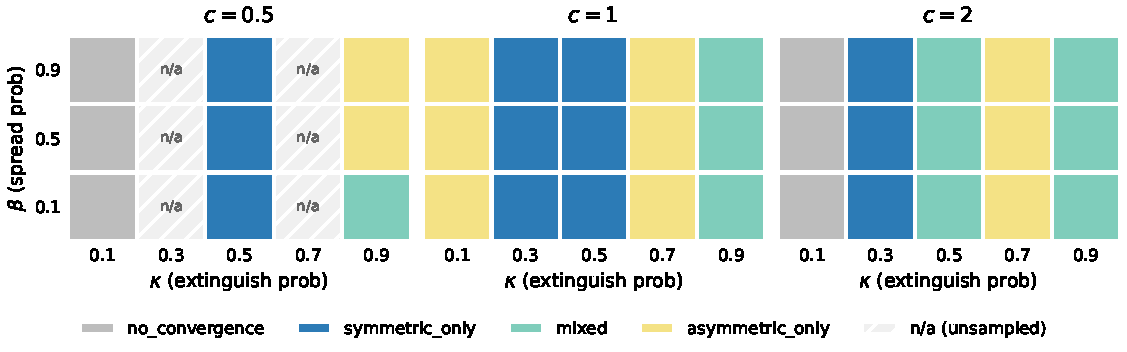
\includegraphics[width=\linewidth]{figures/phase_diagram.pdf}
  \caption{Empirical NE phase diagram for 4-agent Bucket Brigade
  across $(\beta,\kappa,c)$ at $\rho{=}0.02,T_{\min}{=}12$ under the
  \texttt{minimal\_specialization} reward tuple. Each cell is the
  verdict of a heterogeneous Double-Oracle solver over the continuous
  heuristic-parameter strategy space (Hero, Firefighter, FreeRider,
  $\ldots$); the six unsampled cells (high-$\kappa\times c{=}0.5$
  corner, subsumed by the $c{=}1.0$ row) are hatched. Four regimes
  appear across the grid: \textsf{no\_convergence} at low~$\kappa$
  (collapse), \textsf{symmetric\_only} at moderate~$\kappa$ (Hero NE
  dominates), \textsf{asymmetric\_only} at
  high~$\kappa,c{\lesssim}1$ (1 Hero + 3 Firefighters; the rest-trap),
  and a fourth \textsf{mixed} regime (both pure NE coexist) primarily
  at $\kappa{=}0.9,c{\geq}1$. The grid is approximately
  $\beta$-independent at the verdict level (12 of 13 $(\kappa,c)$ rows
  identical across $\beta$; the lone splitting row is
  $(\kappa{=}0.9, c{=}0.5)$). Note that in the bernoulli extinguish
  mode used here the environment is bit-identical across $\beta$
  (repo issue~\#442), so the $\beta$ axis functions as a solver-noise
  probe rather than a test of~\eqref{eq:S}--\eqref{eq:C}; the
  $\kappa$ thresholds remain substantially different from where the
  closed-form derivation places them.}
  \label{fig:phase}
\end{figure}

\section{Trainability: PPO against the NE phase diagram}
\label{sec:trainability}

\paragraph{Protocol.}
We trained independent PPO runs on each of $37$ phase-diagram cells from
Figure~\ref{fig:phase} using the in-repo \texttt{JointPPOTrainer} on the
\texttt{minimal\_specialization} scenario, with $50$ training iterations of
$2048$ rollout steps and $4$ random seeds per cell ($N{=}148$ runs). Two
cells (\verb|b0.10_k0.50_c0.50|, \verb|b0.10_k0.90_c0.50|) were skipped in
the sweep---the $\beta{=}0.1,c{=}0.5$ column at $\kappa\in\{0.5,0.9\}$ was
not scheduled---leaving 37 of the 39 Nash-solver cells with PPO data.
Hyper-parameters are pinned in \texttt{experiments/p3\_specialization/}; the
sweep ran on a single 16-core host (\texttt{alc-2}) in approximately six
hours. The PPO implementation follows the standard recipe
of~\citet{ppo2017}; the multi-agent joint-policy formulation follows the
MAPPO-style centralised-critic setup of~\citet{mappo2022}. The cells
from Appendix~\ref{app:nestructure} contribute the NE verdict for each
$(\beta,\kappa,c)$ combination tested.

\paragraph{Per-cell NE-anchored metric.}
The original v1 sweep scored every cell against a single canonical baseline
(the \texttt{Random} and \texttt{SpecialistPolicy} returns measured at one
calibration cell, $\beta{=}0.25,\kappa{=}0.5$). That metric was misleading
across cells because the random-policy return varies substantially with
$\kappa$ (a low-$\kappa$ cell is intrinsically harder for any policy, so a
small absolute gap against the canonical-cell baseline understates relative
PPO success). We replaced it with $\texttt{gap\_closed\_ne}$, the per-cell
gap-closure ratio between Random and the NE \emph{policy profile}
recovered for that cell by the heterogeneous Double-Oracle solver
(typically $1\times$\texttt{Hero}~$+~3\times$\texttt{Firefighter} on
asymmetric-only and mixed cells, and $4\times$\texttt{Hero} on
symmetric-only cells). The per-cell baselines are tabulated in
\texttt{experiments/nash/phase\_diagram/per\_cell\_baselines.json} and
computed by \texttt{bucket\_brigade/baselines/per\_cell.py}; the recipe is
the same Random/SpecialistPolicy methodology of Appendix~\ref{app:nestructure},
applied per cell. The methodological lesson is independent of this paper's
specific claims: single-cell baselines mislead cross-cell PPO comparison
whenever the random-policy return is itself a function of the cell's
parameters, and per-cell calibration is the necessary correction. We report
this as a separate contribution alongside the data themselves.

\paragraph{Results.}
Figure~\ref{fig:ppo} reports the per-cell $\texttt{gap\_closed\_ne}$
(mean$\pm$std over 4 seeds) across the three~$c$ panels. The ordering across
NE classes is
\textsf{symmetric\_only}~$(0.180;n{=}11)$~$>$~%
\textsf{mixed}~$(0.107;n{=}9)$~$>$~%
\textsf{asymmetric\_only}~$(0.059;n{=}11)$~$>$~%
\textsf{no\_convergence}~$(-0.049;n{=}6$; the metric falls back to
$\texttt{gap\_closed\_homogeneous}$ because no NE policy exists$)$,
consistent with the analytical prediction for the three classes the
bound covers and placing the empirically-observed \textsf{mixed} class
between \textsf{symmetric\_only} and \textsf{asymmetric\_only}---the
location consistent with both pure NE being available but neither being
the unique attractor. We report the ordering, not statistical
significance: the per-class mean within-cell std
($\approx 0.21$--$0.44$) is larger than the corresponding
class-mean separations on $\texttt{gap\_closed\_homogeneous}$
($0.001, 0.017, 0.082$; we use the homogeneous separations here for
metric consistency since no-convergence cells lack
$\texttt{gap\_closed\_ne}$), so the data is consistent with the
predicted ordering but does not reject the null of equal class means
under a standard test. A cross-class $4{\times}$-budget sweep is in
scope for the camera-ready and is the natural significance gate.
$\beta$-invariance holds at verdict level on all $13$ $(\kappa,c)$ rows
of the PPO subgrid with~$\geq 2$ $\beta$ samples (the PPO sweep skipped
the lone splitting Nash row, $(\kappa{=}0.9, c{=}0.5)$); recall from
\S\ref{sec:ne} that the environment is bit-identical across $\beta$ in
this extinguish mode (repo issue~\#442), so cross-$\beta$ variation in
the PPO metric at fixed $(\kappa,c)$ cannot reflect differences in game
dynamics and instead bounds the run-to-run noise of the training
pipeline itself~--~a reading we exploit in the negative-result
paragraphs below. PPO recovers substantial value on
symmetric-only cells, partial value on mixed and asymmetric-only cells,
and approximately none on no-convergence cells, consistent with the
hypothesis that PPO converges reliably when a clean symmetric attractor
exists, struggles when the only NE requires symmetry-breaking, and fails
when no pure-strategy NE is available to converge to.

\paragraph{Is PPO failure on no-convergence cells budget-limited?}
We ran a $4{\times}$-budget sweep on the six no-convergence cells
($200$ iterations $\times$ $4096$ rollout steps, $4$ seeds, $\approx 6$ hours
on \texttt{alc-6}): mean $\texttt{gap\_closed\_homogeneous}$ worsens to
$-0.108$ (from $-0.049$ at the original budget). PPO's failure on
no-convergence cells is therefore structural, not budget-limited; longer
training spends more rollouts in the absence of a pure-strategy attractor
and per-seed runs drift further from the cell-specific
\texttt{SpecialistPolicy} baseline. The load-bearing claim is the direction
of the shift; we report the absolute magnitudes as they fall out.

A methodological observation we report as a separate contribution:
under the original single-cell baseline of the v1 draft, the 7-cell
preview ordering inverted to
\textsf{asymmetric\_only}~$(0.262)$~$>$~\textsf{symmetric\_only}~$(0.091)$~$>$~%
\textsf{no\_convergence}~$(-0.176)$, which would have falsified the
\S\ref{sec:ne} prediction. The inversion is an artefact of the metric:
asymmetric-only cells at $\kappa{=}0.9$ have a much lower random-policy
return than the canonical baseline cell, so PPO's \emph{absolute}
improvement looked large despite recovering a smaller fraction of the
available NE value. Per-cell baselines resolve the ambiguity and the
corrected ordering matches the analytical prediction on both the 7-cell
preview and the full~$37$-cell sweep.

\paragraph{Per-cell trainability predictors: a negative result.}
The class-level ordering above invites a stronger question: does some
scalar property of a cell's NE structure predict how much of the gap PPO
closes in \emph{that cell}? The first candidate we proposed---the
conditional entropy of the cell's converged heterogeneous NE
profile---is retired. Across the $31$ cells with a converged NE
baseline, per-cell mean conditional entropy against
$\texttt{gap\_closed\_ne}$ gives Spearman $\rho{=}0.007$ ($p{=}0.97$);
all four entropy aggregates (mean, max, min, spread) are insignificant
against both $\texttt{gap\_closed\_ne}$ and
$\texttt{gap\_closed\_homogeneous}$, and the single nominally
significant entry (spread vs.\ homogeneous, $p{=}0.039$) does not
survive Bonferroni correction for the eight tests in the family
($\alpha{=}0.0063$). The joined data, statistics, and generating script
are committed at
\texttt{experiments/nash/phase\_diagram/entropy\_vs\_trainability.\{py,json,md\}}.

The failure is structural, not specific to entropy. Within each
$(\kappa,c)$ column of the grid the converged NE profile---and hence
\emph{any} statistic computed from it---is identical across $\beta$
(indeed the environment itself is bit-identical across $\beta$ in this
extinguish mode; \S\ref{sec:ne}), while
$\texttt{gap\_closed\_ne}$ varies across $\beta$ by up to $0.36$ within
a column (e.g.\ $-0.32/-0.11/-0.00$ at $\kappa{=}0.1,c{=}1.0$). The
within-column trainability variance is therefore unexplainable by any
function of the NE profile, entropy or otherwise. Two further readings
follow: per-cell trainability prediction requires inputs beyond the
equilibrium profile, and at $n{=}4$ seeds the per-cell std of
$\texttt{gap\_closed\_ne}$ reaches $0.99$ (median $0.24$)---a noise
ceiling that caps the achievable correlation for \emph{any} predictor
tested against these means.

\paragraph{The noise ceiling, bought down at $20$ seeds.}
A $20$-seed noise buy-down on an $8$-cell subset spanning the four NE
classes (repo issue~\#443; identical training budget, seeds $46$--$61$
added to the committed $42$--$45$;
\texttt{experiments/nash/phase\_diagram/noise\_buydown\_precision.md})
quantifies and partially lifts that ceiling. The $95\%$
percentile-bootstrap CI half-widths on per-cell mean
$\texttt{gap\_closed\_ne}$ shrink by $2.00$--$3.64{\times}$
(median $2.65$; $1.84$--$3.59{\times}$ on
$\texttt{gap\_closed\_homogeneous}$)---consistent with the
$\sqrt{5}\approx 2.24$ expected from $5{\times}$ the seeds, so the
buy-down bought precision, not just seeds. At the higher precision,
\emph{none} of the $8$ re-measured trainability-ladder verdicts flips
(all remain \textsf{insufficient}), and the entropy retirement above
survives recomputation with the $n{=}20$ means substituted (Spearman
$\rho{=}0.109$, $p{=}0.56$; all four aggregates insignificant). The
$n{=}4$ point estimates were noise-dominated but directionally
right---the largest per-cell shift is $0.372\to 0.043$ at
$(\kappa{=}0.3, c{=}1.0)$---so the conclusions drawn from the $n{=}4$
means stand while their error bars, as flagged above, did not deserve
trust.

\paragraph{The coordination-threshold hypothesis (validation pending).}
Our working replacement hypothesis is the coordination threshold
$k^{*}$: the minimum coalition size whose simultaneous deviation from
uniform play yields a positive team-return gap, with the conjecture that
PPO trains where $k^{*}{=}1$ and fails where coordinated multi-agent
deviation is required. We state this as a hypothesis, not a finding.
The $20$-seed buy-down above enables a first class-comparison test
under a \emph{partial} $k^{*}$ stratification (two cells proven
$k^{*}{\geq}2$ by a downstream oracle,
\texttt{rjwalters/thrust\#259}/\texttt{\#268}; six $k^{*}{=}1$
candidates): the separation on $\texttt{gap\_closed\_homogeneous}$ is
not significant (exact one-sided Mann--Whitney $p{=}0.43$; exhaustive
$28$-assignment permutation $p{=}0.39$)---though with class sizes $2$
vs.\ $6$ the minimum achievable one-sided $p$ is ${\approx}0.036$, so
the test has little power and this is an absence of evidence, not
evidence of absence. The full test (all $13$ effective cells, actual
$k^{*}$ values, the $\texttt{gap\_closed\_ne}$ column where defined)
remains blocked on the per-cell $k^{*}$ artifact
(\texttt{rjwalters/thrust\#269}, open). The account must also contend with an awkward datum: a
scripted $k{=}1$ best response against three frozen uniform opponents
already finds a decisive team-return improvement ($+13.4$/step over
uniform, paired 95\% CI $[+10.5, +16.6]$, i.e.\ ${\approx}14\%$) on the
$c{=}0.5$
\textsf{no\_convergence} cells where PPO stays flat
(\texttt{experiments/nash/phase\_diagram/improvability\_oracle.md}), so
single-agent improvability alone does not separate trainable from
untrainable cells. This paper accordingly makes no quantitative
predictor claim; the retirement of the entropy predictor (re-verified
at $n{=}20$) and the $\beta$-invariance impossibility argument are the
results we stand behind.

\paragraph{Caveats.}
The original-budget sweep covers $37$ of the $39$ Nash cells; within-class
statistics ($n{=}11$ symmetric, $n{=}9$ mixed, $n{=}11$ asymmetric,
$n{=}6$ collapse) are wider than the v1 preview but modest for any
significance-style claim, hence the explicit ordering-not-significance
framing of the Results paragraph above. The PPO budget per cell is
modest by recent MARL standards. The $\texttt{gap\_closed\_homogeneous}$
metric (per-cell Random~$\to$~SpecialistPolicy~$\times$~4) reports
smaller cross-cell separation but yields the same qualitative ordering
on the $37$-cell sweep
(\textsf{symmetric}~$(0.051)$~$>$~\textsf{mixed}~$(0.050)$~$>$~%
\textsf{asymmetric}~$(0.033)$~$>$~\textsf{collapse}~$(-0.049)$), so the
load-bearing claim is robust to the metric choice.

\begin{figure}[t]
  \centering
  
\includegraphics[width=\linewidth]{figures/recalibrated_heatmap.pdf}
  \caption{Per-cell PPO $\texttt{gap\_closed\_ne}$ on the $37$-cell sweep
  ($4$ seeds per cell; $50$ iterations $\times$ $2048$ rollout steps with
  the in-repo \texttt{JointPPOTrainer}), arranged in three panels by
  cost~$c\in\{0.5,1.0,2.0\}$. Mean shown above the Tufte-style horizontal
  bar; bar half-width is proportional to per-cell std (4 seeds), scaled so
  the widest std spans 80\% of the cell. Symmetric-only cells (top-left
  of each panel) show the largest gap closure; asymmetric-only cells (top-
  and middle-right) show positive but smaller gap closure; \textsf{mixed}
  cells fall between; \textsf{no\_convergence} cells (bottom row;
  hatched, $\dagger$ marker) report $\texttt{gap\_closed\_homogeneous}$
  instead---values are near zero or negative. On
  \textsf{no\_convergence} cells the
  $\texttt{gap\_closed\_ne}$ metric is undefined because no
  NE policy profile exists; $\texttt{gap\_closed\_homogeneous}$
  (per-cell Random~$\to$~SpecialistPolicy~$\times$~4) is the natural
  fallback because the all-Hero \texttt{SpecialistPolicy} is the
  strongest stationary policy available on those cells, even though it
  is not a NE. Two cells ($\beta{=}0.1$ at
  $\kappa\in\{0.5,0.9\}, c{=}0.5$, n/a, hatched light grey) were skipped
  by the sweep schedule. The ordering across NE classes is consistent
  with the analytical prediction of \S\ref{sec:ne}.}
  \label{fig:ppo}
\end{figure}

\section{Social-trap hardness: measured headroom PPO does not capture}
\label{sec:resttrap}

The phase-diagram cells of \S\ref{sec:trainability} all derive from the
\texttt{minimal\_specialization} scenario, where the equilibrium profile
is also a strong team outcome. Bucket Brigade additionally ships a
scenario engineered so that the equilibrium is team-suboptimal by
construction---a social trap---and on that scenario the benchmark can
make a hardness statement that, to our knowledge, no surveyed benchmark
makes with committed measurements: \emph{at the standard training
budget every trained policy is statistically indistinguishable from
random play; at $16{\times}$ budget exactly one configuration separates
from random---marginally, and with no improvement in the mean---while a
hand-coded scripted team demonstrates ${\approx}80$/step of headroom
that no trained configuration approaches.}

\paragraph{The scenario and its anchors.}
\texttt{rest\_trap-v1} (frozen scenario ID; 4 agents) has a frozen
heterogeneous NE of $3{\times}$\texttt{FreeRider}~$+$~%
$1{\times}$\texttt{Firefighter} with team payoff $2984.04$/episode,
i.e.\ at most $248.67$/step at the $12$-night minimum episode length
(\texttt{bucket\_brigade/baselines/release/local/nash/rest\_trap-v1.json}).
That bound sits \emph{below} the $302.87$/step uniform-random baseline:
rational play is collectively worse than noise. Two caveats keep this
honest. First, per the \S\ref{sec:ne} solver-noise caveat (repo
issue~\#442), the frozen NE \emph{payoff} carries unquantified
double-oracle solver noise (a battery-seeded symmetric-oracle retry,
below, searched for a better equilibrium and found nothing that
stands); the trap \emph{ordering} is nonetheless robust, because the
fully scripted \texttt{always\_rest} team also scores below random
($288.55$/step, 95\% CI $[285.20, 291.65]$). Second, the equilibrium
payoff is per-episode while the anchors are per-step; the
$\leq 248.67$/step bound is conservative in the direction that matters
for the trap claim. Table~\ref{tab:trap-anchors} collects the measured
anchor ladder.

\begin{table}[h]
  \centering
  \small
  \setlength{\tabcolsep}{5pt}
  \begin{tabular}{lll}
    \toprule
    Anchor & Per-step team reward & Provenance \\
    \midrule
    Frozen NE ($3{\times}$FR$+1{\times}$FF) & $\leq 248.67$
      & frozen NE payoff $2984.04$/ep $\div$ $12$ nights \\
    \texttt{always\_rest} $\times 4$ (scripted) & $288.55$ $[285.20, 291.65]$
      & scripted battery screen, $n{=}2000$ \\
    Uniform random & $302.87$; $302.94$ $[301.46, 304.31]$ at $n{=}10$k
      & committed baseline; re-measured upper bound \\
    \texttt{het\_ppo}, standard budget ($20$ seeds) & $306.26$ $[302.95, 309.33]$
      & trailing-5 mean, seed-bootstrap 95\% CI \\
    \texttt{het\_ppo}, $16{\times}$ budget ($20$ seeds) & $307.83$ $[305.00, 310.71]$
      & budget-scaling ladder; first \textsf{escaped\_trap} \\
    \texttt{specialist} $\times 4$ (scripted best) & $\mathbf{386.60}$ $[386.17, 387.03]$
      & all-scripted battery, $n{=}10$k paired episodes \\
    \bottomrule
  \end{tabular}
  \caption{Measured anchor ladder on \texttt{rest\_trap-v1} (per-step
  team reward). The equilibrium and full resting both score below
  random---the trap is real---while a hand-coded homogeneous
  \texttt{specialist} team beats uniform random by $+83.67$/step
  (paired 95\% CI $[+82.36, +84.89]$, $n{=}10{,}000$ paired episodes),
  demonstrating the scenario is not reward-capped at random-level play.
  The $16{\times}$-budget \texttt{het\_ppo} row is the lone trained
  configuration whose CI lower bound clears the random anchor's
  measured upper bound ($305.00$ vs.\ $304.31$); see the budget-scaling
  paragraph for why that flip is variance-driven, not a mean
  improvement. Sources:
  \texttt{experiments/p3\_specialization/scripted\_battery/rest\_trap.\{json,md\}},
  \texttt{experiments/p3\_specialization/tier1\_runs/tier1\_verdict.md},
  \texttt{experiments/p3\_specialization/tier1\_runs\_trap\_escape/}.}
  \label{tab:trap-anchors}
\end{table}

\paragraph{Symmetric-oracle cycling is a property of the scenario, not
a hole in the characterization.}
Earlier revisions of this paper hedged that the symmetric double-oracle
solve for \texttt{rest\_trap} had never converged, leaving open whether
a better (symmetric) equilibrium existed. A battery-seeded retry (repo
issue~\#445;
\texttt{experiments/nash/rest\_trap\_seeded\_do/RESULTS.md}) settles
the question. With the scripted-battery winners---including the
$386.60$/step specialist---injected into the oracle's initial pool, the
symmetric double oracle ran its full $50$-iteration budget without
approaching convergence: minimum per-iteration improvement $11.79$
against a threshold of $\varepsilon{=}0.01$, equilibrium payoff
oscillating in $[1611.56, 2316.61]$/episode with no trend---the same
basin as the earlier unseeded run---so cycling is not a
seeding-coverage artifact; the cooperative region was proposed from
iteration~$1$ and the solver moved away from it. Both candidate
profiles the run surfaces are measurably far from equilibrium: the final
mixed profile is exploitable by at least $407.50$/episode (best
deviation \texttt{always\_rest}---the trap in miniature; rest-leaning
deviations gain, work-leaning deviations lose), and the genome image of
the scripted specialist team is exploitable at every position ($+605$
to $+870$/episode). Nothing found in either run beats the frozen
asymmetric NE ($3{\times}$\texttt{FreeRider}~$+$~%
$1{\times}$\texttt{Firefighter}, $2984.04$/episode), which stands as
the scenario's characterization: at the measured exploitability bounds
\texttt{rest\_trap} admits no symmetric equilibrium---role
differentiation is required---and symmetric-oracle non-convergence is
the symmetric-solver view of that fact, now documented as a property of
the game rather than an open hole. (The cycling mechanism itself is
solver noise: at the verification budget the final solve's
``indifferent'' support strategies actually score from $-258$ to
$+237$/episode against the mixture, so each new best response reshuffles
the support.) This closes the repository's equilibrium coverage at
$12/12$ frozen scenarios: $11$ converged symmetric equilibria plus
\texttt{rest\_trap} as an explicitly non-converged,
exploitability-annotated entry with the asymmetric NE standing.

\paragraph{Why the fraction ladder is inapplicable here---and a vacuous
historical pass.}
The $\texttt{gap\_closed}$ fraction metric of \S\ref{sec:trainability}
needs an upper reference that beats its lower reference; on a social
trap the equilibrium sits below random, so no valid upper reference
exists and the fraction ladder is degenerate (repo issue~\#434 makes
this scenario-aware in the scoring tool:
$\texttt{gap\_source}{=}\texttt{degenerate\_reference}$,
$\texttt{gap\_closed}{=}\texttt{null}$). Before that correction, tier-1
runs on \texttt{rest\_trap} were scored against
\texttt{minimal\_specialization}-scale references, under which a
uniform-random policy alone mapped to $\texttt{gap\_closed}\approx 6.58$
and \emph{any} policy, trained or not, passed the $0.49$ gate. Every
historical ``pass'' recorded for \texttt{rest\_trap} under that gate was
therefore vacuous, and no such result---including in earlier internal
write-ups of this project---should be read as evidence that a trainer
escaped the trap.

\paragraph{Categorical trap-escape verdict.}
The replacement rule (repo issue~\#436;
\texttt{run\_tier1\_cell.classify\_trap\_verdict}) computes the
percentile bootstrap 95\% CI $[lo, hi]$ over seeds of the trained
trailing-5 per-step team reward ($10{,}000$ resamples, fixed RNG seed)
and walks a nested one-sided ladder on $lo$:
$lo > \texttt{scripted\_best.ci95\_hi}$~$\to$~\textsf{above\_scripted\_best};
$lo > \texttt{random\_ci95\_hi}$~$\to$~\textsf{escaped\_trap};
$lo > \texttt{ne\_bound}$~$\to$~\textsf{at\_random}; else
\textsf{trapped\_at\_ne}. The \textsf{escaped\_trap} rung deliberately
anchors on the random baseline's \emph{measured} 95\% upper bound
($304.31$ at $n{=}10$k), not the bare $302.87$ point, which carries
${\pm}1.4$/step measurement noise: a sub-noise clearance of the point is
not a statistically supportable ``above random'' claim.

\paragraph{The honest trained-policy result at the standard budget:
\textsf{at\_random}.}
The strongest standard-budget tier-1 result on \texttt{rest\_trap-v1}
is heterogeneous
PPO (\texttt{het\_ppo}, per-agent policies, $20$ seeds): trailing-5 mean
$306.26$, seed-bootstrap CI $[302.95, 309.33]$~$\to$~verdict
\textsf{at\_random}. The CI lower bound clears the random \emph{point}
by $0.08$/step but not the random anchor's own measured upper bound, so
\texttt{het\_ppo} cannot be ruled significantly above random; the
quantitative headline is
$\texttt{uplift\_over\_random}{=}{+}3.39\pm 7.34$/step. It does clear
the NE bound---PPO does not fall \emph{into} the resting trap---while
capturing essentially none of the ${\approx}80$/step measured scripted
headroom. The hypothesis that per-agent policy asymmetry rescues
learning on asymmetric-equilibrium scenarios therefore currently has
\emph{no} positive interventional evidence on this benchmark (the
marginal $16{\times}$-budget result below does not supply it either,
for the reasons given there); we state
this explicitly so that the retracted vacuous gate pass above is not
read as such evidence. For context, the tier-1 trainer battery on
\texttt{minimal\_specialization-v1} (\texttt{ippo}, \texttt{influence},
\texttt{hca}, \texttt{lola}; $3$ seeds each) scores
\textsf{insufficient} on the fraction ladder
($\texttt{gap\_closed}$ mean $0.005$--$0.125$), so the gap is not an
artifact of one weak trainer
(\texttt{experiments/p3\_specialization/tier1\_runs/tier1\_verdict.md}).

\paragraph{Budget scaling: a marginal statistical escape at
$16{\times}$, with no mean improvement.}
Is the at-random plateau a training-budget artifact? A pre-registered
budget-scaling ladder (repo issue~\#444; stopping rule: end the ladder
at the first \textsf{escaped\_trap}) re-ran \texttt{het\_ppo} and
\texttt{ippo} at $4{\times}$ and $16{\times}$ the tier-1 budget
($200$/$800$ iterations $\times$ $2048$ rollout steps, $20$ seeds per
cell;
\texttt{experiments/p3\_specialization/tier1\_runs\_trap\_escape/}).
Three of the four cells remain \textsf{at\_random} ($4{\times}$
\texttt{het\_ppo} CI lower bound $304.03$; $4{\times}$/$16{\times}$
\texttt{ippo} $301.77$/$303.46$); \texttt{het\_ppo} at $16{\times}$
produces the first \textsf{escaped\_trap} verdict recorded for any
trainer on \texttt{rest\_trap-v1}: trailing-5 mean $307.83$,
seed-bootstrap 95\% CI $[305.00, 310.71]$, lower bound clearing the
$304.31$ random-anchor upper bound by $+0.69$/step. The crossing is
robust to the test machinery---the CI lower bound clears the anchor
under $300/300$ combinations of bootstrap RNG seed and resample count,
and a non-bootstrap $t$-interval on the $20$ seed means,
$[304.67, 310.99]$, clears it as well---but it must be read for what
it is. \emph{There is no dose-response on the mean}: the plateau is
flat across budgets ($306.26 \to 307.66 \to 307.83$; all paired
same-seed contrasts insignificant, e.g.\
$16{\times}{-}1{\times} = {+}1.57 \pm 4.80$/step, $t{=}1.46$),
extending the $4{\times}$ vanilla-PPO flatness of
\S\ref{sec:trainability} to \texttt{het\_ppo}, \texttt{ippo}, and
$16{\times}$. \emph{The verdict flip is variance-driven}: extra budget
tightens the seed spread (uplift std $8.36 \to 6.59$), marching the CI
lower bound up ($302.95 \to 304.03 \to 305.00$) around an essentially
unchanged mean---budget buys seed-level consistency, not performance.
And \emph{the learnability gap stands}: the mean uplift
(${+}4.96$/step) is ${\approx}6\%$ of the measured $83.7$/step scripted
headroom, and the best single seed anywhere in the ladder captures
${\approx}27\%$ of it, remaining ${\approx}61$/step below
\texttt{scripted\_best}. Two caveats travel with the row: the four
ladder cells share seed streams, so they are CRN-coupled rather than
independent tests, and one of four 95\%-CI tests crossing by
$0.69$/step is weak stand-alone evidence---the verdict rule is
pre-registered, so the row stands as scored, as \emph{marginally but
significantly above random}, never as ``PPO solves the trap at
scale.'' The ladder also supplies the sharpest interventional contrast
to date for the per-agent-asymmetry hypothesis---\texttt{het\_ppo}
crosses the escape threshold where \texttt{ippo} at the identical
budget does not---but the two trainers' means are statistically
indistinguishable, so we do not count that as positive evidence
either. Net effect: the hardness headline of this section is
unchanged and, if anything, sharpened---$16{\times}$ compute buys
statistical separation from random and no progress toward the
specialist solution.

The resulting benchmark statement is unusually concrete: on
\texttt{rest\_trap-v1} the target is not ``do better''; it is a
committed, machine-verdicted ladder
(${\leq}248.67 < 302.87 < 307.83 < 386.60$ per step) in which the
\textsf{escaped\_trap} rung has now been reached exactly once,
marginally, by $16{\times}$-budget heterogeneous PPO, and the remaining
${\approx}79$/step gap to \texttt{scripted\_best} is known to be
realizable by a stationary policy profile. The open challenge is no
longer statistical separation from random play; it is capturing
headroom.

\section{Related work}
\label{sec:related}

The MARL community has converged on a handful of canonical benchmarks that
trade equilibrium transparency for environment richness.
Overcooked-AI~\citep{overcooked2019} is a fully cooperative coordination
game on small grid layouts: every Pareto-optimal joint policy is a Nash
equilibrium and ``the'' target is therefore not unique. Melting
Pot~\citep{meltingpot2021} exposes 88$\times$88$\times$3 RGB observations
across more than 50 substrates; its design explicitly does not solve for
equilibrium structure on individual substrates. The Hanabi
Challenge~\citep{hanabi2020} has near-optimal hat-guessing strategies known
at 2 players, but the 4--5 player game is open and no algorithm reaches the
equilibrium from learning. SMAC and SMACv2~\citep{smac2019,smacv2_2023} are
cooperative micromanagement against a scripted opponent and ``NE'' is not a
design target. MAgent~\citep{magent2018} hosts thousand-agent battles on
grids and no published equilibrium analysis exists at scale.
PettingZoo's MPE suite~\citep{pettingzoo2021} is the canonical small
multi-agent baseline with no equilibrium characterisation across scenarios.

Table~\ref{tab:bench} compares Bucket Brigade against these on six axes.

\begin{table}[t]
  \centering
  \small
  \setlength{\tabcolsep}{3pt}
  \resizebox{\linewidth}{!}{%
  \begin{tabular}{lrrrcl}
    \toprule
    Benchmark & Year & Agents & Per-agent $|\mathcal{A}|$ & NE characterisable? & Coop/comp \\
    \midrule
    Overcooked-AI~\citep{overcooked2019}      & 2019      & 2        & 6          & No (any Pareto-opt.) & coop \\
    Melting Pot~\citep{meltingpot2021}        & 2021      & 2--16    & 8          & No (intractable)     & mixed \\
    Hanabi~\citep{hanabi2020}                 & 2020      & 2--5     & $\leq 20$  & Partial (2P only)    & coop \\
    SMAC/SMACv2~\citep{smac2019,smacv2_2023}  & 2019/23   & 2--27    & 6+$n_e$    & No                   & vs.\ scripted \\
    MAgent~\citep{magent2018}                 & 2018      & 64--$10^3$ & 21       & No (population)      & mixed \\
    PettingZoo MPE~\citep{pettingzoo2021}     & 2021      & 2--6     & 3--5       & No                   & per-scenario \\
    \textbf{Bucket Brigade (this work)}       & 2026      & 4 (def.) & 8 / 40     & \textbf{Yes (closed-form)} & \textbf{mixed within cell} \\
    \bottomrule
  \end{tabular}%
  }
  \caption{Bucket Brigade against the six most-cited canonical MARL
  benchmarks. The right-most column ``NE characterisable?'' is the only
  axis on which Bucket Brigade dominates; on every other axis the
  surveyed benchmarks are richer, more cited, or larger in scope. This is
  the entire pitch: Bucket Brigade is a \emph{methodological complement},
  not a replacement. Per-agent action sizes for Bucket Brigade are
  $8$ at the $H{=}2$ minimal scenario and $40$ at the $H{=}10$ default.}
  \label{tab:bench}
\end{table}

The honest comparison is that Bucket Brigade dominates on exactly one
column---NE characterisability---and loses on every other (citation
footprint, agent count, environment richness, generality). The paper's job
is to argue that the NE-characterisability column matters enough to be worth
introducing a new benchmark despite the trade. Bucket Brigade does not
scale to large populations, does not test ``emergent cooperation'' in
any general sense, and is not a general-purpose MARL benchmark. The
niche it fills is the specific question of
\emph{equilibrium-convergence quality}.

\section{Discussion and limitations}
\label{sec:discussion}

\paragraph{Bucket Brigade is intentionally small and artificial.}
The state space is~$2304$ at the minimal scenario and $\sim\!10^{10}$ at the
default 10-house scenario, the geometry is a 1-D ring, and the environment
ships from a single research repository with no community adoption. We
acknowledge each point head-on and defend it as the cost of the
equilibrium-transparency property:
(a)~\emph{Size is the cost of NE transparency.} A richer game with realistic
observations, partial observability across many channels, and complex spatial
dynamics would lose the property that motivated the work; the state-space
cardinality is what makes the analytical reduction in~\S\ref{sec:ne}
algebraically tractable. Trading richness for tractability is the deliberate
design choice.
(b)~\emph{A custom benchmark is acceptable given the methodological niche.}
The question we want to answer---``did this MARL algorithm converge to the
analytically-characterised NE?''---cannot be asked of any of the six
canonical benchmarks in Table~\ref{tab:bench}. A benchmark designed for this
question is therefore a methodological contribution distinct from the
contributions those benchmarks make, even if it does not inherit their scale
or citation impact.
(c)~\emph{Bucket Brigade is not a substitute for any of the six.} It does
not replace Overcooked for human-AI coordination, Melting Pot for
generalisation across substrates, Hanabi for partial-observability
cooperation, SMAC for micromanagement against scripted opponents, MAgent
for population-scale phenomena, or PettingZoo for the small-multi-agent
baseline role. A researcher choosing a benchmark for any of those purposes
should not pick Bucket Brigade.

\paragraph{Threats to the contributions.}
On the analytical side, the closed-form thresholds disagree with
empirics by 3--10$\times$ in $\kappa$-threshold location
(\S\ref{sec:ne}), and the bound does not predict the empirical
\textsf{mixed} class at the higher-$c$ rows. The three identified
systematic biases---ring locality, per-agent ownership rewards, and the
heuristic-strategy approximation---are not separated by the existing
grid; rigorous separation requires a sweep in which $\beta$ is actually
live (the contagion-active phase order or the continuous-extinguish
variant of Appendix~\ref{app:envspec:variants}---in the bernoulli mode
used here $\beta$ is provably inert, so no $\rho$-sweep can activate it;
repo issue~\#442), and a
ring-Markov refinement of the survival coefficient $A$ to predict the
\textsf{mixed} boundary in closed form. Whether the solver's converged
asymmetric profiles are themselves $\varepsilon$-NE under
common-random-number re-evaluation is an open thread (repo
issue~\#459). On the empirical side, per-class
sample size is modest ($n\in\{6,9,11,11\}$) and the budget per run is
modest; the $4{\times}$-budget sweep rules out one budget-limited
hypothesis for the no-convergence row but not the cross-class question,
which is in scope for the camera-ready, and the $20$-seed noise
buy-down of \S\ref{sec:trainability} lifts the per-cell seed-noise
ceiling on $8$ of the $37$ cells (verdicts unchanged) without yet
covering the rest of the grid. The per-cell-baseline
methodological result of \S\ref{sec:trainability} stands independently
of both the longer-budget outcome and the ring-Markov refinement: it is
load-bearing on cross-cell PPO comparison whenever the random-policy
return varies across cells, regardless of the analytical reduction's
fate.

\paragraph{Reproducibility.}
The environment is shipped as a pip-installable Python package
(\texttt{pip install bucket-brigade}); the figure-by-figure reproduction
recipe lives in the in-repo \texttt{docs/PAPER\_RESULTS.md}. The per-cell
baselines used by the \S\ref{sec:trainability} metric are produced by
\texttt{bucket\_brigade/baselines/per\_cell.py} and serialised at
\texttt{experiments/nash/phase\_diagram/per\_cell\_baselines.json}; both
ship with the repository so the recalibrated $\texttt{gap\_closed\_ne}$
column of Figure~\ref{fig:ppo} can be re-derived from the raw PPO-sweep
checkpoints. (The v2 recalibrated artifacts this paper reports
reproduce byte-for-byte from the committed per-seed summaries; a
reproduction drift in the \emph{superseded} v1 tables is tracked openly
as repo issue~\#461.)

Three pieces of infrastructure added after the sweeps target the failure
mode benchmark consumers actually hit. \emph{Frozen scenario IDs}: every
scenario this paper reports on carries a versioned, immutable registry
entry (\texttt{minimal\_specialization-v1}, \texttt{rest\_trap-v1}, and
the registered phase-diagram cells such as
\texttt{asym\_b05\_k09\_c05-v1}), guarded by bit-parity regression tests
(\texttt{bucket\_brigade/envs/registry.py}; repo PR~\#441). Numbers in
this paper cite frozen IDs, never bare scenario names. \emph{Parity
manifest and check}: a committed manifest records, per frozen scenario,
the canonical uniform-random per-step team reward with its $n{=}1000$
bootstrap CI and a scenario-parameter fingerprint; a seconds-cheap CLI
(\texttt{python -m bucket\_brigade.baselines.parity --all}) re-measures
an installed build against the manifest with a CI-derived tolerance and
fails loudly on mismatch (\texttt{docs/PARITY.md}; repo PR~\#439).
\emph{The motivating incident}: a downstream harness ran a full study of
this benchmark on a differently-weighted reward configuration whose
returns were ${\sim}7{\times}$ repo-native scale; nothing failed loudly,
and the mismatch was only exposed by a dedicated repo-side scripted
oracle (repo PR~\#432). Results produced off-scale are worse than no
results; the parity check converts that class of silent mismatch into an
immediate failure, and we ask anyone publishing numbers about Bucket
Brigade to cite the frozen scenario ID, the manifest version, and a
passing parity check.

Frozen baseline checkpoints (the analytical \texttt{Hero},
\texttt{Firefighter}, and \texttt{FreeRider} agents used to anchor the
phase-diagram solver and the per-cell PPO metric) will be hosted on the
HuggingFace Hub; the publication pathway for the baselines is in progress
and not yet complete at the time of this draft. The source repository is at
\url{https://github.com/rjwalters/bucket-brigade}.

\section*{Conclusion}

We presented Bucket Brigade, a parametric cooperative-competitive MARL
benchmark whose Nash-equilibrium structure is characterisable in closed form
across a smooth three-scalar parameter family. A single-house mean-field
reduction yields algebraic boundary inequalities~\eqref{eq:S}--\eqref{eq:C}
that correctly predict the qualitative phase order on the full~$39$-cell
grid (its $\beta$-independence prediction, while correct, holds by
construction in the sweep's bernoulli extinguish mode and now serves as
a solver-noise probe rather than a confirmation), while disagreeing with
empirics on the quantitative
$\kappa$-thresholds by 3--10$\times$ and failing to predict a fourth
empirical \textsf{mixed} class at the higher-$c$ rows---a gap we own and
attribute to the named systematic biases. The $37$-cell PPO trainability
sweep, evaluated under a per-cell NE-anchored metric, recovers the
predicted ordering
\textsf{symmetric}~$>$~\textsf{mixed}~$>$~\textsf{asymmetric}~$>$~%
\textsf{collapse}; a separate $4{\times}$-budget sweep on the
no-convergence cells worsens gap-closure, indicating PPO's failure on those
cells is structural, not budget-limited. The per-cell NE-anchored metric is itself a
standalone methodological finding: on this paper's data the previously-used
single-cell baseline inverted the per-class ordering, so per-cell
calibration is necessary, not cosmetic, for any cross-cell PPO comparison
in which the random-policy return varies across cells. At the per-cell
level we report a negative result---conditional entropy of the NE
profile does not predict gap closure, and no statistic of the NE profile
can, by the $\beta$-invariance argument of
\S\ref{sec:trainability}---re-verified by a $20$-seed noise buy-down
that shrinks CI half-widths $2.0$--$3.6{\times}$ and flips none of the
$8$ re-measured verdicts, with the coordination-threshold $k^{*}$
hypothesis still unvalidated (its class test is insignificant under a
partial, low-power stratification and the full test is blocked on a
pending per-cell $k^{*}$ artifact). On the
social-trap scenario \texttt{rest\_trap-v1}, the benchmark's hardest
committed target, the equilibrium characterization is now closed (the
asymmetric NE stands; two independent symmetric-oracle runs cycle, and
the seeded run's outputs carry measured exploitability bounds), trained
policies at the standard budget are statistically
indistinguishable from random play, and a $16{\times}$-budget ladder
yields exactly one marginal, variance-driven statistical escape with no
improvement in the mean---budget buys precision, not
performance---while a scripted specialist team
demonstrates ${\approx}80$/step of realizable headroom---a
machine-verdicted learnability gap we offer as a concrete challenge.
Bucket Brigade is positioned as a methodological
complement to the canonical MARL benchmarks for the specific question of
equilibrium-convergence quality, not as a replacement for any of them.

\bibliographystyle{plainnat}
\bibliography{refs}

\appendix

\section{Formal environment specification}
\label{app:envspec}

This appendix gives the self-contained mathematical contract for the Bucket
Brigade environment. \S\ref{sec:env} of the body is a compressed summary;
the material below is what a reader needs to reimplement the environment
from scratch in any language, with the seven-phase ordering, the
independent-workers extinguish formula, and the per-agent reward
decomposition all spelled out. The notation matches \S\ref{sec:env}
verbatim.

\subsection{Players and parameters}
\label{app:envspec:setup}

\paragraph{Player set.} A finite set of agents
$\mathcal{I}=\{1,2,\ldots,N\}$, with $N\geq 1$ fixed across an episode.
Agents are \emph{positionally symmetric}: the environment dynamics are
invariant under any permutation $\sigma:\mathcal{I}\to\mathcal{I}$ applied
jointly to every per-agent quantity (locations, signals, actions,
rewards). The asymmetric reward variants of~\S\ref{app:envspec:variants}
(per-agent home-position cost, per-agent ownership weights) break this
symmetry only when their dedicated parameters are nonzero; the symmetric
default game preserves exchangeability.

\paragraph{Topology.} The world is a cycle graph
$\mathcal{H}=\mathbb{Z}/H\mathbb{Z}$ with $H\geq 2$ vertices (``houses'')
and edge set $\{(h,h{+}1\bmod H):h\in\mathcal{H}\}$. House indices are
taken mod $H$ throughout. The two neighbours of house $h$ are
$h{-}1\bmod H$ and $h{+}1\bmod H$.

\paragraph{Parameter family.} The full parameter family is
$\theta=(\beta,\kappa,\rho,c,H,N,T_{\min},W)$ where $\beta\in[0,1]$ is the
per-night, per-neighbour fire-spread probability; $\kappa\in[0,1]$ is the
per-agent solo extinguish probability; $\rho\in[0,1]$ is the per-night,
per-\textsc{Safe}-house spontaneous-ignition probability; $c\in\mathbb{R}_{\geq 0}$
is the per-night work cost; $H\in\mathbb{Z}_{\geq 2}$ is the number of
houses; $N\in\mathbb{Z}_{\geq 1}$ is the number of agents;
$T_{\min}\in\mathbb{Z}_{\geq 0}$ is the minimum nights before termination
is allowed; and $W$ is the reward tuple of~\S\ref{app:envspec:reward}.

The default ``10-house'' scenario uses $H{=}10,N{=}4,\beta{=}0.25,
\kappa{=}0.5,\rho{=}0.02,c{=}0.5,T_{\min}{=}12$ and reward weights
$W=(R_{\text{team}},P_{\text{team}},r_{\text{own}},r_{\text{other}},
p_{\text{own}},p_{\text{other}})=(100,100,20,0,40,0)$. The minimal
parameterisation sets $H{=}2,N{=}4$.

\subsection{State, action, observation}
\label{app:envspec:soa}

\paragraph{State.} The environment state at the start of night $t$ is
\[
  s_t = (h_t,\ell_t,\zeta_t,t)\in\{S,B,R\}^H\times
        \mathcal{H}^N\times\{0,1\}^N\times\mathbb{N},
\]
where $h_t\in\{S,B,R\}^H$ is the vector of house statuses (\textsc{Safe},
\textsc{Burning}, \textsc{Ruined}), $\ell_t\in\mathcal{H}^N$ is the
vector of agent locations, $\zeta_t\in\{0,1\}^N$ is the vector of one-bit
broadcast signals emitted on the previous night, and $t\in\mathbb{N}$ is
the night counter. The \textsc{Ruined} status is absorbing; \textsc{Safe}
and \textsc{Burning} are mutually reachable.

\paragraph{Initial state.} At $t{=}0$ each house is independently
\textsc{Burning} with probability $\rho$ and \textsc{Safe} otherwise;
agent locations are $\ell_{0,i}{=}0$ and signals $\zeta_{0,i}{=}0$ for
all $i$.

\paragraph{State cardinality.}
$|\{S,B,R\}^H\times\mathcal{H}^N\times\{0,1\}^N|=3^H\cdot H^N\cdot 2^N$.
For $H{=}2,N{=}4$ this is $9\cdot 16\cdot 16=2304$ states; for
$H{=}10,N{=}4$ it is $\approx 9.44\times 10^{9}$. The state space is
polynomial in $(H,N)$ rather than exponential in observation pixels.

\paragraph{Action.} Each agent $i$ chooses an action $a_{t,i}=
(a_{t,i}^{\text{house}},a_{t,i}^{\text{mode}},a_{t,i}^{\text{sig}})$
from the product set $\mathcal{A}=\mathcal{H}\times\{0,1\}\times\{0,1\}$,
with $a^{\text{house}}\in\mathcal{H}$ the target house index,
$a^{\text{mode}}\in\{0,1\}$ the \textsc{Work} bit ($1$~=~\textsc{Work},
$0$~=~\textsc{Rest}), and $a^{\text{sig}}\in\{0,1\}$ the broadcast bit
emitted this night and observable to all agents on the next. Per-agent
cardinality is $|\mathcal{A}|=4H$ ($8$ at $H{=}2$, $40$ at $H{=}10$);
joint-action cardinality is $|\mathcal{A}^N|=(4H)^N$ ($4096$ at
$H{=}2,N{=}4$). The signal bit is strictly informational, incurs no
cost, and does not constrain the agent's mode or location; signals
support cheap-talk equilibria but the interpretation is not part of the
specification.

\paragraph{Observation.} The environment is perfect-monitoring with
one-step delay on signals: at the start of night $t$, every agent
observes the same tuple
$o_t=(h_t,\ell_{t-1},\zeta_{t-1},\alpha_{t-1},t)$, where
$\alpha_{t-1}\in\mathcal{H}^N\times\{0,1\}^N$ is the previous night's
joint $(\text{house},\text{mode})$ slice. There is no partial
observability of houses or agent positions and no private observations.

\subsection{Transition dynamics}
\label{app:envspec:dynamics}

A single night consists of seven sequential phases applied to the state.
The phase order is load-bearing: swapping any two adjacent phases changes
the transition kernel. The order is (1)~signal write, (2)~location and
mode write, (3)~extinguish, (4)~burn-out, (5)~spread, (6)~spontaneous
ignition, (7)~reward and termination check. Write
$w_h(a):=|\{i:a_i^{\text{house}}=h\land a_i^{\text{mode}}=1\}|$ for the
number of agents who \textsc{Work} at house $h$ under joint action $a$.

\paragraph{Signal and bookkeeping (phases 1--2).}
$\zeta_t\leftarrow(a_{t,i}^{\text{sig}})_{i\in\mathcal{I}}$,
$\ell_t\leftarrow(a_{t,i}^{\text{house}})_{i\in\mathcal{I}}$. These
updates do not alter house states.

\paragraph{Extinguish phase (phase 3).}
For each house $h$ with $h_{t,h}=B$, draw $U\sim\mathrm{Uniform}[0,1]$
and update
\[
  h_{t,h}^{(3)} = \begin{cases}
    S & \text{if } U < 1-(1-\kappa)^{w_h(a_t)} \\
    B & \text{otherwise}
  \end{cases}
\]
The independent-workers extinguish formula: each \textsc{Work}er at the
house independently succeeds with probability $\kappa$, so at least one
succeeds with probability $1-(1-\kappa)^{w_h}$. \textsc{Safe} and
\textsc{Ruined} houses are unaffected.

\paragraph{Burn-out phase (phase 4).}
Every house that survived the extinguish phase as \textsc{Burning}
transitions deterministically to \textsc{Ruined}:
$h_{t,h}^{(4)}=R$ if $h_{t,h}^{(3)}=B$, else $h_{t,h}^{(4)}=h_{t,h}^{(3)}$.

\paragraph{Spread phase (phase 5).}
For each pair $(h,h')$ with $h_{t,h}^{(4)}=B$, $h'\sim h$ on the ring,
and $h_{t,h'}^{(4)}=S$, draw independent $U\sim\mathrm{Uniform}[0,1]$
and set $h_{t,h'}^{(5)}=B$ if $U<\beta$. Under the canonical phase
order, phase 4 has already cleared every \textsc{Burning} source house
to \textsc{Ruined}, so phase 5 is inert in the canonical mode and the
only path \textsc{Safe}~$\to$~\textsc{Burning} during a night is the
spontaneous-ignition phase 6. A contagion-active variant swaps phases 4
and 5; under that variant a \textsc{Safe} house with two \textsc{Burning}
neighbours has combined ignition probability $1-(1-\beta)^2$. The
phase-diagram analysis in the body uses the canonical order.

\paragraph{Spontaneous ignition phase (phase 6).}
For each house $h$ with $h_{t,h}^{(5)}=S$, draw independent
$U\sim\mathrm{Uniform}[0,1]$ and set $h_{t,h}^{(6)}=B$ if $U<\rho$.
\textsc{Ruined} houses are unaffected; freshly-\textsc{Ruined} houses
from phase 4 cannot re-ignite. The resulting state is
$h_{t+1}:=h_t^{(6)}$.

\subsection{Reward structure}
\label{app:envspec:reward}

Rewards are paid at the end of each night, after all transition phases.
The per-agent reward $r_{t,i}$ decomposes into three independently
parameterised terms.

\paragraph{Work/rest term.}
$r_{t,i}^{\text{work}}=-c$ if $a_{t,i}^{\text{mode}}=1$
(\textsc{Work}), and $+c_{\text{rest}}$ if $a_{t,i}^{\text{mode}}=0$
(\textsc{Rest}), with $c_{\text{rest}}=0.5$ as the implementation
default. \textsc{Rest} is a positive payoff that opt-in \textsc{Work}
forgoes; the free-rider gradient is the $c+c_{\text{rest}}$ asymmetry.

\paragraph{Per-house ownership term.}
Each house $h$ has a designated owner $\mathrm{owner}(h)\in\mathcal{I}$
assigned at episode start by round-robin: $\mathrm{owner}(h)=h\bmod N$.
The per-house contribution to agent $i$'s reward is
\[
  r_{t,i,h}^{\text{own}} = \mathbb{1}[h_{t-1,h}\neq S\land h_{t+1,h}=S]
                           \cdot w^{\text{save}}_i(h)
                         - \mathbb{1}[h_{t+1,h}=R]\cdot w^{\text{ruin}}_i(h),
\]
with weights
\[
  w^{\text{save}}_i(h) = \begin{cases}
    r_{\text{own},i} & i=\mathrm{owner}(h) \\
    r_{\text{other},i} & \text{otherwise}
  \end{cases},\qquad
  w^{\text{ruin}}_i(h) = \begin{cases}
    p_{\text{own},i} & i=\mathrm{owner}(h) \\
    p_{\text{other},i} & \text{otherwise.}
  \end{cases}
\]
The save event fires once on the night the house transitions from
non-\textsc{Safe} to \textsc{Safe}; the ruin penalty fires every night
the house remains \textsc{Ruined}, so a ruined house imposes a recurring
cost until the episode terminates.

\paragraph{Team-welfare term.}
Let $n_S(t):=|\{h:h_{t+1,h}=S\}|$ and $n_R(t):=|\{h:h_{t+1,h}=R\}|$.
The team term, paid to every agent equally, is
$r_t^{\text{team}}=R_{\text{team}}\cdot n_S(t)/H
                  -P_{\text{team}}\cdot n_R(t)/H$.

\paragraph{Total reward.}
$r_{t,i} = r_{t,i}^{\text{work}}
         + \sum_{h\in\mathcal{H}} r_{t,i,h}^{\text{own}}
         + r_t^{\text{team}}$.

\subsection{Horizon, information, symmetries, variants}
\label{app:envspec:variants}

\paragraph{Termination.}
The episode terminates at night $T$ when $t\geq T_{\min}$ \emph{and} at
least one of the following holds: all houses are \textsc{Safe}, all
houses are \textsc{Ruined}, or no house is \textsc{Burning}. Under
canonical parameters with $\rho>0$ the no-fires-burning condition holds
only transiently, so termination typically occurs via the absorbing
all-\textsc{Ruined} condition or via a transient \textsc{Safe} state that
survives the spontaneous-ignition draw. Expected episode length is
finite for $\rho>0$, but the game is not strictly finite-horizon.

\paragraph{Information structure.}
The information structure is symmetric perfect monitoring: every agent
observes the full state $h_t$, the previous joint
location/mode/signal $(\ell_{t-1},\alpha_{t-1}^{\text{mode}},
\zeta_{t-1})$, and the night counter $t$. No agent has private
information about house states or other agents' actions. The signal
channel is non-binding cheap talk: $\zeta_{t,i}$ is observable to every
agent at night $t{+}1$ but is functionally decoupled from
$a_{t+1,i}^{\text{mode}}$.

\paragraph{Symmetry properties.}
The default game enjoys agent exchangeability (the transition kernel and
reward function are invariant under any permutation $\sigma$ of agent
indices) and ring rotation (the transition kernel is invariant under any
rotation $\tau:h\mapsto h+k\bmod H$ applied jointly to $h_t,\ell_t,
a_t^{\text{house}}$; reward invariance requires ownership weights to be
permuted consistently with $\tau$). Asymmetric reward variants break
agent exchangeability; the position-constrained variant breaks ring
rotation by anchoring each agent to a home position.

\paragraph{Optional dynamic variants.}
Four optional variants are part of the calibrated parameter family, each
gated by a parameter that defaults to the no-op value: (a)~adjacent-only
action validity (per-agent home position $h^{\text{home}}_i$ with a
ring-distance-${\leq}1$ constraint on $a_i^{\text{house}}$);
(b)~continuous-extinguish (each \textsc{Work} at a \textsc{Burning} house
adds increment $\sigma$ to a per-house accumulator; the fire transitions
to \textsc{Safe} deterministically when the accumulator reaches 1; fires
do not burn out); (c)~two-phase signalling (each night becomes two
micro-rounds with round-1 emitting signal only and round-2 observing
everyone's round-1 signal); (d)~distance-cost asymmetry (work cost
augmented to $c+\alpha\cdot d(h^{\text{home}}_i,a_i^{\text{house}})$
where $d$ is ring-arc distance, breaking ring-rotation symmetry).
These variants are out of scope for the paper but are part of the broader
calibrated family.

\subsection{Relationship to canonical game-theory templates}
\label{app:envspec:templates}

Bucket Brigade recovers, as limiting cases or restrictions, several
textbook templates.

\paragraph{Volunteer's Dilemma.}
At $N{=}1,H{=}1$ with $\rho>0,\beta{=}0$, each night the single agent
faces a binary choice: \textsc{Work} (pay $c$, save the house with
probability $\kappa$) or \textsc{Rest} (gain $c_{\text{rest}}$, lose the
house in the next phase). This is the textbook single-shot Volunteer's
Dilemma. The $N$-player generalisation at $N>1,H=1$ is the
\emph{$N$-player Volunteer's Dilemma}: the team needs at least one
volunteer per fire, with the free-rider incentive equal to the
$c+c_{\text{rest}}$ gap.

\paragraph{$N$-Player Public Goods Game.}
With $r_{\text{own}}=r_{\text{other}}$ and $p_{\text{own}}=p_{\text{other}}$
(ownership weights collapsed to uniform), the per-house ownership term
reduces to a non-excludable common good and the team term is paid equally
regardless of contribution. The marginal private return to \textsc{Work}
is then $\kappa\cdot(R_{\text{team}}+P_{\text{team}})/H-c$, which can be
strictly less than the social marginal return $\kappa\cdot
(R_{\text{team}}+P_{\text{team}})-c$, producing the textbook public-goods
underinvestment gradient.

\paragraph{Stag Hunt.}
In the limit $\kappa\to 1$ a single worker is sufficient to extinguish
any fire, but the work cost $c$ remains. The game then has two natural
NE: the all-stag cooperative NE where every agent works coordinated
houses (high payoff, requires coordination beliefs) and the all-hare
lazy NE where everyone \textsc{Rest}-defects (low payoff, no coordination
required). The intermediate-$\kappa$ regime interpolates between Stag
Hunt and the public-goods regime.

\paragraph{Free-rider problem (rest-trap).}
At specific parameter cells the unique pure-strategy NE is asymmetric:
$N{-}1$ agents play \textsc{Rest} and one agent plays full-force
\textsc{Work}. This is the textbook free-rider problem in the
bucket-brigade vocabulary; the phase diagram across $(\beta,\kappa,c)$
shows the boundary between symmetric-NE-dominant and
asymmetric-NE-dominant regimes.

\paragraph{Stochastic Game.}
Stripped to its bones, Bucket Brigade is a finite-state, finite-action,
discounted stochastic game with $N$ players, symmetric perfect
monitoring, and reward decomposition into private and team components.
Every formal result for finite stochastic games---minimax, equilibrium
existence in stationary mixed strategies, value iteration
convergence---applies directly. The contribution of the Bucket Brigade
design is not in the game-theoretic class but in the \emph{size}: at the
minimal parameterisation the game is small enough that standard tools
actually compute, which is the property the paper exploits.

\subsection{Notation summary}
\label{app:envspec:notation}

\begin{table}[h]
  \centering
  \small
  \setlength{\tabcolsep}{4pt}
  \begin{tabular}{ll}
    \toprule
    Symbol & Meaning \\
    \midrule
    $\mathcal{I}=\{1,\ldots,N\}$ & Agent set; $N$ = population size \\
    $\mathcal{H}=\mathbb{Z}/H\mathbb{Z}$ & House ring; $H$ = number of houses \\
    $S,B,R$ & House statuses: \textsc{Safe}, \textsc{Burning}, \textsc{Ruined} (R absorbing) \\
    $\beta$ & Per-night, per-neighbour fire-spread probability \\
    $\kappa$ & Solo-agent extinguish probability (independent-workers model) \\
    $\rho$ & Per-night, per-\textsc{Safe}-house spontaneous-ignition probability \\
    $c$ & Per-night work cost (paid when $a_i^{\text{mode}}=1$) \\
    $c_{\text{rest}}$ & Per-night rest payoff (implementation default 0.5) \\
    $T_{\min}$ & Minimum nights before termination allowed \\
    $a_{t,i}=(a^{\text{house}},a^{\text{mode}},a^{\text{sig}})$
      & Per-agent action: target house, work bit, signal bit \\
    $w_h(a)$ & Number of \textsc{Work}ers at house $h$ under joint action $a$ \\
    $R_{\text{team}},P_{\text{team}}$
      & Team reward / penalty per fraction-safe / fraction-ruined \\
    $r_{\text{own}},r_{\text{other}}$
      & Per-agent save-reward weights (own / other-owned house) \\
    $p_{\text{own}},p_{\text{other}}$
      & Per-agent ruin-penalty weights (own / other-owned house) \\
    $n_S(t),n_R(t)$ & Counts of \textsc{Safe} / \textsc{Ruined} houses at end of night $t$ \\
    $\zeta_t\in\{0,1\}^N$ & Vector of broadcast signals (observable next night) \\
    $\ell_t\in\mathcal{H}^N$ & Vector of agent locations after phase 2 \\
    \bottomrule
  \end{tabular}
  \caption{Notation summary. Every downstream section (\S\ref{sec:ne}
  equilibrium analysis, \S\ref{sec:trainability} experiments,
  \S\ref{sec:discussion} discussion, Appendix~\ref{app:nestructure} NE
  derivation) reuses this vocabulary without redefinition.}
  \label{tab:notation}
\end{table}

\paragraph{Reproducibility note.} The seven-phase ordering of
\S\ref{app:envspec:dynamics} is load-bearing: implementers must apply
phases in the exact order (signal write, location/mode write,
extinguish, burn-out, spread, spontaneous ignition, reward). The
independent-workers extinguish formula of~\S\ref{app:envspec:dynamics}
and the post-extinguish, pre-burn-out spread test are the two details
most often misread on first encounter; both are explicit above to make
reimplementation tractable. A reader who reimplements from this
appendix alone---using any RNG and any programming language---should
obtain matching equilibrium structure and policy-evaluation results at
the documented parameter cells.

\section{Analytical NE characterisation for the 4-agent game}
\label{app:nestructure}

This appendix gives the full derivation of the closed-form boundary
inequalities reported in~\S\ref{sec:ne} and the predicted-vs-empirical
comparison table referenced in Figures~\ref{fig:phase}
and~\ref{fig:ppo}. The derivation reduces the $H{=}10$ ring with
$T_{\min}{=}12$ to a one-house, four-agent, single-night stage game
whose payoffs absorb multi-step contagion and ignition dynamics into a
single survival coefficient. The three NE structures fall out as
algebraic inequalities in $(\kappa,\tilde A,c_{\text{gap}})$.

\subsection{Setup}
\label{app:nestructure:setup}

The analysis is restricted to the \texttt{minimal\_specialization}
parameter cell with $H{=}10,N{=}4,T_{\min}{=}12$ and reward tuple
$W=(R_{\text{team}},P_{\text{team}},r_{\text{own}},r_{\text{other}},
p_{\text{own}},p_{\text{other}})=(10,10,50,0,100,0)$ at $\rho{=}0.02$.
The free parameters are $(\beta,\kappa,c)$.

The analytical reduction is \emph{not} a derivation of the full
stochastic-game subgame-perfect equilibrium. The full game's NE
conditions exist only via numerical value iteration on the
$\geq 9\times 10^{9}$-state space, which does not generalise across
$(\beta,\kappa,c)$ in closed form. Restricting to the per-night stage
game under stationary opponent strategies is the load-bearing
simplification that makes algebraic boundary inequalities possible;
\S\ref{app:nestructure:gaps} reports where this restriction produces
visibly wrong predictions.

\paragraph{Mapping to the empirical strategy space.}
The empirical phase diagram is computed by the heterogeneous
Double-Oracle solver over continuous 10-D heuristic-parameter vectors,
not the binary \textsc{Work}/\textsc{Rest} stage game the derivation
uses. The bridge is the work-tendency parameter: \texttt{Hero}
(\texttt{work\_tendency}${=}1.0$) maps to analytical all-\textsc{Work};
\texttt{Firefighter} (\texttt{work\_tendency}${=}0.9$) is treated as
near all-\textsc{Work}; \texttt{FreeRider}
(\texttt{work\_tendency}${=}0.2$, \texttt{rest\_reward\_bias}${=}0.9$)
maps to all-\textsc{Rest}. Empirical verdicts map to analytical NE
structures as: \textsf{symmetric\_only} with profile
$4{\times}$\texttt{Hero}~$\to$~symmetric all-\textsc{Work};
\textsf{asymmetric\_only} with profile
$1{\times}$\texttt{Hero}~$+~3{\times}$\texttt{Firefighter}~$\to$
asymmetric 1-\textsc{Worker}; \textsf{no\_convergence}~$\to$ no-pure-NE
collapse. The mapping is approximate---\texttt{Firefighter}s at
\texttt{work\_tendency}${=}0.9$ are not literal \textsc{Rest}
agents---and the quantitative bias this introduces is named
in~\S\ref{app:nestructure:gaps}.

\paragraph{Single-house mean-field reduction.}
Instead of analysing the full 10-house ring with 4 agents distributed
across houses, we collapse the analysis to a representative single house
with all 4 agents present, where the night's outcome is paid out as the
expected per-agent payoff under the stage-game profile. Per-night
reward decomposition follows~\S\ref{app:envspec:reward}: a work cost
$-c$ on \textsc{Work} and rest payoff $+c_{\text{rest}}{=}0.5$ on
\textsc{Rest}; a per-house ownership term weighted by
$r_{\text{own}}{=}50$ on save and $p_{\text{own}}{=}100$ on every
\textsc{Ruined} night; and a team term scaled by
$R_{\text{team}}{=}P_{\text{team}}{=}10$. In the single-house reduction
ownership accrues to the house's designated owner and is shared equally
across agents in the steady-state assumption that each agent owns one
house and the rotation is symmetric.

\subsection{Mean-field stage-game reduction}
\label{app:nestructure:reduction}

\paragraph{Survival coefficient.}
With $k\in\{0,1,2,3,4\}$ workers at the house on a given night, the
probability of extinguish in phase 3 is $1-(1-\kappa)^k$. Under the
canonical phase order the spread phase has no \textsc{Burning} source
houses to spread from, so $\beta$ does not enter the leading-order
single-night payoff and contagion enters only via spontaneous ignition
at rate $\rho$ per \textsc{Safe} house. Let $s$ be the probability a
house is \textsc{Safe}; conditional on \textsc{Safe} at night $t$ and
$k$ workers on night $t{+}1$, the per-night ruin probability is
\[
  q(k) := 1 - \Pr[s_{t+1}{=}S\mid s_t{=}S,k] = \rho\cdot(1-\kappa)^k.
\]
Over $T_{\min}{=}12$ nights the probability the house survives is
approximately $(1-q(k))^{T_{\min}}\approx 1-T_{\min}\cdot q(k)$ for small
$q(k)$. Collecting the $q(k)$-dependent terms of the expected per-house
reward yields
\[
  \mathbb{E}[\text{per-house reward loss}\mid k]
  = A\cdot\rho\cdot(1-\kappa)^k,
\]
with
\[
  A = r_{\text{own}}\cdot T_{\min}
    + p_{\text{own}}\cdot T_{\min}
    + P_{\text{team}}\cdot T_{\min}/H
    = 50\cdot 12 + 100\cdot 12 + 10\cdot 12/10 = 1812.
\]
The marginal benefit of adding the $k$-th worker (going from $k$ to
$k{+}1$) is the reduction in expected loss,
\[
  \Delta(k\to k{+}1)
  = A\cdot\rho\cdot[(1{-}\kappa)^k-(1{-}\kappa)^{k+1}]
  = A\cdot\rho\cdot\kappa\cdot(1-\kappa)^k.
\]
Writing $\tilde A:=A\rho=1812\cdot 0.02=36.24$ for the per-night
survival coefficient, the marginal benefit at the $k$-th worker is
$\tilde A\cdot\kappa\cdot(1-\kappa)^k$.

\paragraph{Stage-game payoffs.}
Each agent picks $a^{\text{mode}}\in\{0,1\}$. With $k_{-i}$ other
workers under the joint profile, agent $i$'s per-night payoff
difference between \textsc{Work} and \textsc{Rest} is
\[
  u_i(\text{Work}\mid k_{-i}) - u_i(\text{Rest})
  = \tilde A\cdot\kappa\cdot(1-\kappa)^{k_{-i}} - c_{\text{gap}},
\]
with $c_{\text{gap}}:=c+c_{\text{rest}}$. For the phase-diagram driver's
$c{=}0.5$ and the default $c_{\text{rest}}{=}0.5$, $c_{\text{gap}}=1.0$.

\paragraph{Ring locality (statement).}
The single-house reduction assumes all 4 agents are at the same house.
The empirical setup spreads 4 agents across 10 houses each night; under
a symmetric uniform policy, each house sees $E[k]=N/H=0.4$ workers per
night. The derivation in~\S\ref{app:nestructure:candidates} keeps the
single-house framing (all 4 agents at one fire) because that is the
case that determines whether a ``1 Worker, 3 free-riders'' profile is
stable; the ring-locality correction is the perturbation in
\S\ref{app:nestructure:gaps}.

\subsection{The three NE candidates}
\label{app:nestructure:candidates}

\paragraph{Symmetric all-\textsc{Work} NE.}
Under the all-\textsc{Work} profile, every agent plays $a_i=\text{Work}$.
For this to be a NE, a unilateral deviation to \textsc{Rest} must not
strictly increase payoff. The deviation comparison has $k_{-i}{=}3$:
\[
  \tilde A\cdot\kappa\cdot(1-\kappa)^3 \geq c_{\text{gap}}
  \qquad\text{(S)}.
\]
Substituting $\tilde A{=}36.24,c_{\text{gap}}{=}1.0$: $f(\kappa):=
\kappa(1-\kappa)^3$ is unimodal on $[0,1]$ with maximum
$f(1/4)=27/256\approx 0.105$. Solving $f(\kappa)=0.0276$
numerically gives roots $\kappa\approx 0.030$ and $\kappa\approx 0.65$;
the symmetric NE exists for $\kappa\in[0.030,0.65]$.

\paragraph{Asymmetric 1-\textsc{Worker} NE.}
Under the asymmetric profile exactly 1 agent \textsc{Work}s and 3
\textsc{Rest}. Two conditions: the lone \textsc{Worker} prefers
\textsc{Work} ($k_{-i}{=}0$) and each free-rider prefers \textsc{Rest}
($k_{-i}{=}1$):
\[
  \tilde A\cdot\kappa\geq c_{\text{gap}}
  \quad\text{AND}\quad
  \tilde A\cdot\kappa\cdot(1-\kappa)<c_{\text{gap}}
  \qquad\text{(A)}.
\]
Condition~(a): $36.24\cdot\kappa\geq 1.0\Leftrightarrow\kappa\geq 0.028$.
Condition~(b): $g(\kappa):=36.24\kappa(1-\kappa)$ is unimodal with
$g(1/2)=9.06$; the roots of $g(\kappa)=1.0$ are $\kappa\approx 0.028$
(lower) and $\kappa\approx 0.972$ (upper). Condition~(b) requires
$\kappa$ outside $[0.028,0.972]$. The intersection of~(a) and~(b) is
essentially empty below $\kappa{=}0.028$ and gives the high-$\kappa$
band $\kappa\gtrsim 0.972$, the Stag-Hunt-like regime where a single
worker is overwhelmingly likely to extinguish and the free-rider's
marginal contribution is negligible.

\paragraph{No-pure-NE collapse.}
The all-\textsc{Rest} profile is never a pure-strategy NE for any
$\tilde A>0$ such that $\tilde A\kappa>c_{\text{gap}}$, because a single
deviation to \textsc{Work} earns $\tilde A\kappa-c_{\text{gap}}>0$. The
no-pure-NE collapse regime is the parameter regime where neither (S)
nor (A) holds AND the all-\textsc{Work} profile is dominated. From the
above, $\tilde A\kappa<c_{\text{gap}}$ implies the lone-\textsc{Worker}
deviation does not pay (A~(a) fails) and a fortiori (S) fails (since
$(1-\kappa)^3<1$ for $\kappa>0$):
\[
  \tilde A\cdot\kappa < c_{\text{gap}}
  \implies \text{no pure-strategy NE (collapse)}
  \qquad\text{(C)}.
\]

\paragraph{Summary table.}
For the \texttt{minimal\_specialization} parameter cell at $c{=}0.5$
(so $c_{\text{gap}}{=}1.0$), $\rho{=}0.02$, $T_{\min}{=}12$, and
$\tilde A=36.24$:

\begin{table}[h]
  \centering
  \small
  \begin{tabular}{lccc l}
    \toprule
    $\kappa$ range & Symmetric~(S) & Asymmetric~(A) & Collapse~(C)
                   & Predicted verdict \\
    \midrule
    $\kappa<0.028$            & No & No & Yes & \textsf{collapse} (no-pure-NE) \\
    $0.028\leq\kappa\leq 0.030$ & Borderline & Empty & No & borderline; may be \textsf{mixed} \\
    $0.030\leq\kappa\leq 0.65$  & Yes & No  & No  & \textsf{symmetric\_only} \\
    $0.65<\kappa\leq 0.972$     & No  & No  & No  & \textsf{mixed} or transition \\
    $\kappa>0.972$              & No  & Yes & No  & \textsf{asymmetric\_only} \\
    \bottomrule
  \end{tabular}
  \caption{Predicted NE structure under the mean-field reduction at
  $c{=}0.5,\rho{=}0.02,T_{\min}{=}12$. The qualitative phase order
  from $\kappa$-small to $\kappa$-large is
  \textsf{collapse}~$\to$~\textsf{symmetric\_only}~$\to$~%
  \textsf{mixed}/no-pure~$\to$~\textsf{asymmetric\_only}, matching the
  empirical ordering on the 39-cell grid at $c{=}0.5$. $\beta$ does not
  enter under the canonical phase order.}
  \label{tab:ne-predicted}
\end{table}

\subsection{Predicted vs.\ empirical phase table (7-cell preview)}
\label{app:nestructure:phasetable}

The 7-cell preview at $c{=}0.5,\rho{=}0.02$ against the predicted
verdict:

\begin{table}[h]
  \centering
  \small
  \begin{tabular}{cclll}
    \toprule
    $\beta$ & $\kappa$ & Empirical verdict & Predicted verdict & Match? \\
    \midrule
    0.10 & 0.10 & \textsf{no\_convergence} & \textsf{symmetric\_only} (in 0.030--0.65 band) & $\times$ \\
    0.50 & 0.10 & \textsf{no\_convergence} & \textsf{symmetric\_only} & $\times$ \\
    0.90 & 0.10 & \textsf{no\_convergence} & \textsf{symmetric\_only} & $\times$ \\
    0.50 & 0.50 & \textsf{symmetric\_only} & \textsf{symmetric\_only} & \checkmark \\
    0.90 & 0.50 & \textsf{symmetric\_only} & \textsf{symmetric\_only} & \checkmark \\
    0.50 & 0.90 & \textsf{asymmetric\_only} & \textsf{mixed}/borderline (predicted threshold $0.972$) & partial \\
    0.90 & 0.90 & \textsf{asymmetric\_only} & \textsf{mixed}/borderline & partial \\
    \bottomrule
  \end{tabular}
  \caption{Predicted vs.\ empirical NE verdict on the 7-cell preview
  reported in~\S\ref{sec:ne} of the body. Qualitative-vs-quantitative
  split: $\beta$-independence holds 3/3 on $\kappa$-rows with both
  $\beta$ values; the qualitative phase ladder
  \textsf{no\_convergence}~$\to$~\textsf{symmetric\_only}~$\to$~%
  \textsf{asymmetric\_only} matches; exact cell-by-cell agreement is
  2/7 because the predicted $\kappa$ thresholds are wrong. The
  predicted collapse threshold $\kappa{=}0.028$ is 3--4$\times$ too
  low; the predicted asymmetric-NE threshold $\kappa{=}0.972$ is
  $\sim 10\%$ too high. The full 39-cell grid in~\S\ref{sec:ne} of the
  body widens the sample without changing the qualitative findings.}
  \label{tab:ne-empirical}
\end{table}

\subsection{Where the reduction breaks}
\label{app:nestructure:gaps}

Five sources of systematic bias are identifiable from the derivation.

\paragraph{Ring locality (the $H{=}10$~$\to$~mean-field gap).}
The reduction puts all 4 agents at one house. Empirically, 4 agents
distribute across 10 houses each night; under a symmetric uniform
policy, each house sees $E[k]=0.4$ workers per night on average rather
than 4. The effective per-house extinguish probability is
$1-(1-\kappa)^{0.4}$ rather than $1-(1-\kappa)^4$---a much weaker
defence. For $\kappa{=}0.5$: full-mean-field gives $1-0.5^4=0.9375$;
the ring-corrected average gives $1-0.5^{0.4}\approx 0.24$. The
ring-corrected $\tilde A$ is therefore much smaller than 36.24, and the
collapse boundary $\kappa$ at which $\tilde A\kappa<c_{\text{gap}}$
shifts substantially upward. Predicted correction: the collapse
threshold moves from $\kappa{=}0.028$ (single-house) to roughly
$\kappa\in[0.1,0.3]$ (ring-corrected), consistent with the empirical
boundary. This is the dominant systematic bias; tightening it without
losing tractability is the open problem.

\paragraph{Heuristic strategy space (\texttt{Firefighter}~$\neq$~all-\textsc{Rest}).}
The empirical solver picks \texttt{Firefighter}s
(\texttt{work\_tendency}${=}0.9$) as the ``free-riders'' in the
asymmetric NE profile, not literal \textsc{Rest}ers
(\texttt{work\_tendency}${=}0.2$). Three \texttt{Firefighter}s at 90\%
\textsc{Work} contribute non-zero expected extinguish probability---the
effective $k_{-i}$ in the lone-\textsc{Worker}'s deviation comparison is
closer to $1+3\cdot 0.9=3.7$ than to the analytical $k_{-i}{=}1$. At
$\kappa{=}0.9$, $\tilde A\kappa(1-\kappa)^{3.7}\approx 0.013\ll
c_{\text{gap}}{=}1.0$, so the lone \textsc{Worker} should not exist as
a NE under that interpretation. The empirical solver still reporting
\textsf{asymmetric\_only} at $\kappa{=}0.9$ suggests the per-agent
ownership reward---not captured in the single-house mean-field
reward---anchors each agent to its own house even when free-riding on
others' fires. The asymmetric NE is therefore partly an artefact of
per-agent ownership, not a pure Volunteer's-Dilemma equilibrium.

\paragraph{Per-agent ownership rewards (the $W$ gap).}
The analytical $A$ coefficient lumps $r_{\text{own}}{=}50$ and
$p_{\text{own}}{=}100$ into the survival term, but the per-agent reward
only fires on the agent's \emph{own} house. The single-house reduction
assumes the representative house is the agent's own house with
probability 1; the ring-corrected reality is probability
$1/H{=}0.1$. The other 9 houses contribute through the team term only,
which scales $A$ down by a factor of roughly
$(p_{\text{own}}/H+P_{\text{team}}/H)/p_{\text{own}}\approx 0.11$ on
the off-own-house terms. The ring-corrected $A$ sits between
$A/H{=}181$ and $A{=}1812$, depending on the agent's house-target
distribution.

\paragraph{$\beta$-independence: exact by construction in bernoulli
mode, not merely leading-order.}
Earlier drafts of this appendix treated $\beta$-independence as a
leading-order approximation that could break via across-night
contagion at large $\beta\rho$. Mechanistic inspection of the engine
(repo issue~\#442) shows that under the canonical phase order in
bernoulli extinguish mode the claim is \emph{exact}: the burn-out
phase (phase~4) transitions every still-\textsc{Burning} house to
\textsc{Ruined} before the spread phase (phase~5) runs, in every
night, so spread never has a \textsc{Burning} source, never fires,
and draws zero RNG. The dynamics \emph{and the RNG stream} are
bit-identical across $\beta$; there is no across-night path for
$\beta$ to enter, and no $\rho$-sweep can activate it. Two
consequences follow. First, the $39$-cell grid's $\beta$ axis carries
no environmental information in this mode~--~a design lesson for
future sweeps, which should either drop the axis or run a variant in
which $\beta$ is live (the contagion-active order that swaps phases
4 and 5, or the continuous-extinguish variant of
\S\ref{app:envspec:variants}). Second, observed cross-$\beta$
differences in solver output at fixed $(\kappa,c)$~--~the splitting
verdict row at $(\kappa{=}0.9,c{=}0.5)$ and payoff deltas such as
$80.9$ vs.\ $72.0$ at that cell and $-614.4$ vs.\ $-648.0$ at
$(\kappa{=}0.5,c{=}0.5)$~--~are pure measurements of double-oracle
solver nondeterminism, usable as a free noise probe.

\paragraph{Single-stage vs.\ multi-stage SPE.}
The reduction is the single-night stage game under stationary opponent
policies, not the full multi-stage subgame-perfect equilibrium.
Empirically, the DO solver evaluates policies over full
$T_{\min}{=}12$ episodes, so per-cell payoffs reflect the integrated
multi-stage outcomes. A symmetric all-\textsc{Work} profile that is a
NE of the single-night stage game may fail to be a NE of the
multi-stage game if a deviator can sustain a long-horizon advantage by
switching to \textsc{Rest} at a specific night. The reduction folds
multi-stage dynamics into $A$ by integrating expected survival over
$T_{\min}$ nights, but the exact multi-stage NE conditions involve
subgame-perfect best-response calculations the single-night reduction
cannot represent.

\subsection{Implications and recommended follow-ups}
\label{app:nestructure:followups}

Even with the quantitative thresholds wrong by 3--10$\times$, the
structural predictions the mean-field reduction makes---(a)
$\kappa$-monotonicity of the verdict and (b) the existence of a
no-pure-NE collapse regime at small $\kappa$---are empirically observed
and would not be derivable without the closed-form derivation. (A third
prediction, (c) $\beta$-independence under the canonical phase order, is
correct but vacuously so in bernoulli extinguish mode, per
\S\ref{app:nestructure:gaps}; it is no longer counted as an empirical
confirmation.) The body of the paper
adopts inequalities (S), (A), (C) as the analytical anchor.

Three concrete follow-ups, in priority order:
(1)~complete the empirical grid across $c\in\{0.5,1.0,2.0\}$ and
re-run the comparison table (now done at the 39-cell scale
of~\S\ref{sec:ne}); (2)~re-run a $\beta$ slice under a variant in which
$\beta$ is live---the contagion-active phase order or the
continuous-extinguish mode of \S\ref{app:envspec:variants}---so the
reduction's $\beta$ treatment can actually be falsified (in bernoulli
mode it cannot be; repo issue~\#442); (3)~derive a ring-Markov correction to
$A$ that replaces the single-house mean-field assumption with a
chain-Markov approximation over the 10-house ring, closing the
\S\ref{app:nestructure:gaps} gap without paying the full state-space
cost.

\end{document}
